% Preamble ------------------------------------------------------------------------

\documentclass[10pt]{article}

 % Package Loads ------------------------------------------------------------------

 \usepackage[utf8]{inputenc}
 \usepackage[T1]{fontenc}
 \usepackage{lmodern}

 \usepackage[letterpaper, total={6.5in, 9in}, footnotesep=0.3in]{geometry}
 \usepackage[colorlinks=true, allcolors=blue]{hyperref}
 \usepackage{sidecap, caption}
 \usepackage{enumitem}
 \usepackage{csquotes}

 \usepackage{graphicx}
 \usepackage{float}

 \usepackage{units}
 \usepackage{amsmath,amsfonts,amssymb}
 \usepackage{gensymb}
 
 \usepackage{titlesec}
 \usepackage{titling}
 \setcounter{secnumdepth}{4}
 \setcounter{tocdepth}{4}
 
 \usepackage{authblk}
 \usepackage[
    natbib=true,
    style=numeric,
    sorting=none
 ]{biblatex}

 
 
 % Path ---------------------------------------------------------------------------

 \graphicspath{{assets/}}
 \addbibresource{bibliography.bib}
 
 % Set Global Font ----------------------------------------------------------------

 \renewcommand{\rmdefault}{lmss}

 % Title Elements -----------------------------------------------------------------
 

 \title{
    {\vspace{-1.5cm}}
    {\hspace{-2cm}}   
    {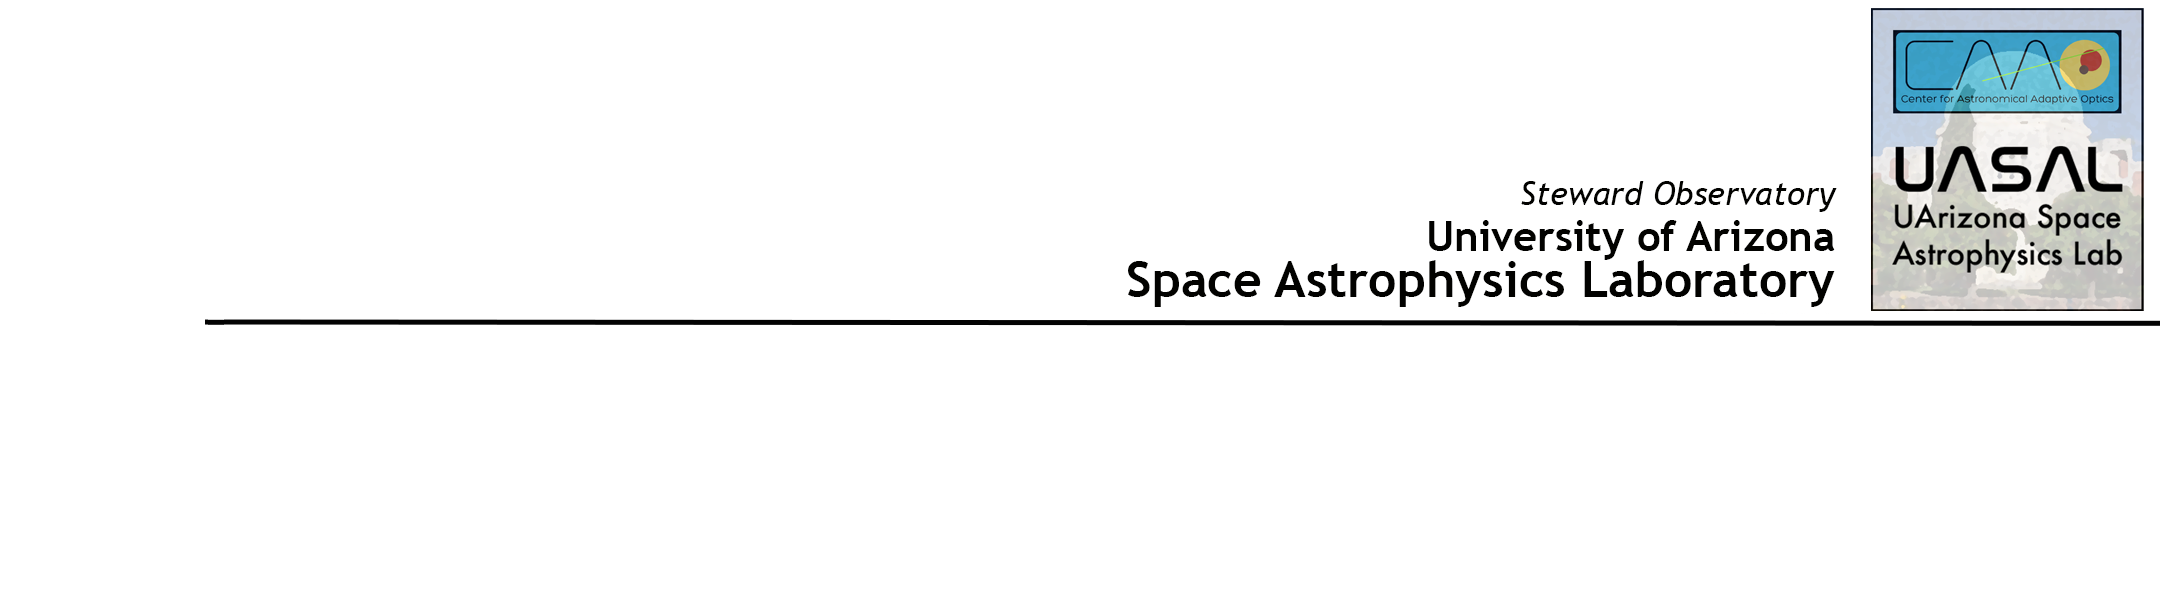
\includegraphics{assets/UASAL_Header.png}}
    {\large }\\
    {Understanding Noise and Noise Reduction in CMOS Imaging Sensors}\\
    {\large \emph{Including Notes on Temporal and Spatial Noise Reduction}}
 } 

 \author{\large Jess Johnson}

 \affil{\small Senior Instrumentation Scientist \\ Steward Observatory, University of Arizona \\ 11 April 2024 \\ \footnotesize Release Version One}

 \date{}

% Document Start ------------------------------------------------------------------

\begin{document}

\fontfamily{lmss}
\maketitle

% Abstract ------------------------------------------------------------------------

\begin{abstract}

In imaging sensors, there are two distinct classes of noise: signal-related noise, which is a function of the impinging photons, independent of the sensor, and sensor-related noise. Sensor noise can be further classified into fixed pattern noise, signal shot noise, and read noise. 

Some of these forms of noise are temporal noise, varying from moment to moment, and others are spatial noise, persistent in time but varying from pixel to pixel. Whereas spatial noise can be effectively mitigated with traditional data reduction techniques, temporal noise, such as electronic noise, is difficult, if not impossible, to effectively reduce. In addition, CMOS sensors are prone to a type of destructive temporal noise known as Random Telegraph Signal Noise, also known as Salt \& Pepper noise, which is extremely difficult to mitigate and increases dramatically over time with exposure to proton radiation. Other forms of noise which are typically of small contribution to the sensor's noise profile at start can also be expected to increase with exposure.

This memo begins with a brief discussion of CMOS structure and architecture, in which the features and structures of active pixel CMOS sensors that are responsible for generating noise are presented. The next section presents a brief overview of the mathematical representation of noise. The following section then lists the classifications8 of CMOS noise, and discusses the various types of noise and the mechanisms that create them.  The next section discusses the combined effects of the different noise sources. The following section breifly touches on the effects of radiation on noise, and the final section deals with noise reduction techniques. The conclusion summarizes the major points of interest to the instrumentation teams.

\newpage

\centerline{\textbf{Author's notes}}

\vspace{5mm}

\emph{This paper was inspired not only by a request from a instrumentation researcher, but also by my need to understand the fundamentals of noise to better inform the design of the sensor testing program, and by my own curiosity and concern.}

\emph{The use of a large number of CMOS sensors in space-based missions is unprecedented, and many aspects of their use in the space environment is not well studied. We do know, from the JUICE mission, that CMOS sensors will degrade in response to radiation, increasing the sensor's noise level. Therefore, understanding noise and its mitigation are extremely important when imaging is used not only for scientific data acquisition, but also for vital functionality such as guidance and wavefront control.}

\emph{This paper is essentially a review of the literature I have digested over the last 18 months of my study of CMOS imaging and the characterization of sensors as it relates to the vital issues of imaging noise and its reduction. No single reference provides a comprehensive overview of all noise sources in a CMOS imager. My role here was to take material from a large number of sources and attempt to organize and present it in a coherent and understandable way. Most of this paper was taken from my notes on those sources, and the largest issue I faced was attempting to filter and compress a voluminous amount of information to the essentials. I made no assumption at the outset about a reader's knowledge level; I begin the discussion from fundamentals.}

\emph{I used three different texts as primary references for this memo. The first is James Janesick's excellent \emph{Photon Transfer: : DN → [lambda]} \emph{\cite{janesick}}. Anyone who wants to more fully understand both CMOS functionality and a powerful method of characterization should read this book. The next is \emph{CMOS Image Sensors}, by Konstantin Stefanov \emph{\cite{stefanov22}}. Although quite technical, it is one of the best 'deep understanding' books on the topic that I've found. The final reference is \emph{Ultra Low Noise CMOS Image Sensors} by Assim Boukhayma \emph{\cite{boukhayma}}. All three of these references complement each other quite well, and all three are highly recommended.}

\emph{There are several important topics briefly discussed here that I continue to pursue, and will report on as necessary. First and most important on that list are white noise and RTS denoising algorithms, which I believe to be essential to allow continued effective operation of CMOS cameras in the space environment. Another important topic is understanding the radiation environment that we will be operating in so that exposure levels to different forms of radiation can be determined over the lifetime of the mission. This will begin to allow us to predict which performance parameters are likely to be degraded, and by how much. This is dependent on the final orbit selection, however, and so sits on the back burner for the time being.}

\vspace{5mm}
\end{abstract}

\newpage

% Table of Contents ---------------------------------------------------------------

\tableofcontents

\newpage

% Section One ---------------------------------------------------------------------

\section{Introduction}

Noise is defined as 'the uncertainty which accompanies [an] acquired signal'\cite{website:teldyne24}. It is an inherent reality in any form of imaging sensor, from photographic to electronic; it is always present as the result of acquiring an image. Some of this noise is a property of light itself, but a significant amount of it originates in the devices that we use to capture the light.

Noise can never be completely eliminated, but by understanding its nature and its origins can be substantially mitigated. The process of characterization, which is the determination of an imager's performance and noise properties, is essential to this endeavor, as it provides critical information as to the extent of noise from various sources that occur in any individual camera. 

The general noise profiles of CCD sensors and CMOS sensors share similarities, and so significant portions of one's knowledge of the noise properties of CCD imagers transfer to understanding noise in CMOS imagers. CMOS does, however, have unique forms of noise that present substantial complications to the typical suite of noise reduction tools, most of which have been developed for working with CCD imagers. In particular, \emph{Random Telegraph Signal noise} (RTS) is a  major issues with CMOS sensors that impacts their use as quantitative imaging devices (see Section~\ref{sec:rtsnoise}), but plays a far lesser role in CCD noise performance.

I should note that there are two types of noise related phenomena that are not covered in this paper. The first, \emph{Fano noise}, is a form of shot noise that occurs in detectors in response to photons with energy levels in the far UV and which becomes of concern in the soft x-ray regime. The second concerns the noise generated by excessive \emph{quantum yield} (QY), specifically the production of multiple photoelectrons per single impinging photon. For silicon, photons of wavelengths between 400 nm and 1200 nm will generate single electrons. As we will be using camera filters passing photons in the 400 nm to 800 nm range, Fano noise is not relevant, and in that range, QY = 1.

\subsection{Classification of Noise Sources}
\label{sec:classification}

There are a bewildering number of places and processes in a CMOS imager in which noise can originate, and therefore many different ways of grouping different noise types into classifications. Let's start with the most basic. and then elaborate as it becomes necessary. 

First, noise is generally divided into two subgroups: \emph{signal noise}, and \emph{sensor noise}. 

\subsection{Signal Noise}

Signal noise is essentially \emph{photon shot noise} (PSN), the result of photons emitted in a fluorescent process forming a light beam whose cross-sectional density follows a Poisson density distribution.  This distribution results from the inherent quantum uncertainty, in both timing and direction, in the emission of photons from an excited source. PSN is proportional to the square root of the signal, and cannot be removed (see Section~\ref{sec:psn}). Its proportionality in the overall noise profile of a sensor decreases with increasing signal strength. Under ideal circumstances, photon shot noise determines the noise floor, a operational condition called \emph{photon shot limited}.

\subsection{Sensor Noise}

The second source of noise, sensor-related noise, is the classification in which all of the other  myriad noise types and mechanisms reside. Some authors and references refer to all sensor noise as \emph{Read Noise}, which is somewhat misleading as not all sensor noise is a function of the readout process. 

There are many sources of noise that arise from the photonic and electrical behavior of CMOS sensors. All of these sources can be grouped together into two further classes, \emph{temporal noise}, or noise which is fundamentally stochastic and varies with time, and \emph{spatial noise}, or noise which is fixed in time but varies across different instances of the same sensor. Spatial Noise is also referred to as \emph{fixed pattern noise}. Within temporal noise, it is common to further subdivide noise types into four more subdivisions, based on where they originate within the imager. These are \emph{dark current noise}, or noise produced by thermal electrons, predominately in the pixel structure itself; \emph {transfer noise}, or noise which originates in a pixel's transfer gate; \emph{electronic noise}, which originates in the imager's electronic circuitry; and \emph{other noise}, a catch-all classification in which to situate noise that doesn't arise from those primary sources.

An outline of noise sources in a CMOS imager looks like this. Following each noise class are the individual types of noise that this paper discusses.

\begin{itemize}[noitemsep]
   \item \textbf{Signal Noise}
       \begin{itemize}[noitemsep]
          \item \textbf{Photon Shot Noise}
       \end{itemize}
   \item \textbf{Temporal Noise}
       \begin{itemize}[noitemsep]
          \item \textbf{Dark Current Noise}
             \begin{itemize}[noitemsep]
                \item Dark Current Shot Noise
                \item Diffusion Dark Current
                \item Deplete Area Generation Noise
             \end{itemize}
          \item \textbf{Transfer Noise}
             \begin{itemize}[noitemsep]
               \item Non-ideal Charge Transfer Noise
          \end{itemize}
          \item \textbf{Electronic Noise}
             \begin{itemize}[noitemsep]
                \item kT/C Noise
                \item MOS Transistor Thermal Noise
                \item 1/f Noise
                \item RTS Noise
                \item Leakage Current Shot Noise
             \end{itemize}
          \item \textbf{Other Noise}
             \begin{itemize}[noitemsep]
                \item ADC Quantizing Noise
                \item System Noise
             \end{itemize}
        \end{itemize} 
   \item \textbf{Spatial Noise}
      \begin{itemize}[noitemsep]
         \item \textbf{Fixed Pattern Noise}
         \begin{itemize}[noitemsep]
                \item Photo Response Non-Uniformity
                \item Offset Spatial Variation
                \item Column Level Gain Variation
                \item Dark Signal Non-Uniformity
                \item Dark Current Fixed Pattern Noise
             \end{itemize}
      \end{itemize}
\end{itemize}

This particular classification scheme is based on the source of the noise, that is, where in the imager it originates. The definitions of each of these noise types, along with the physical processes that create them, are the subject of Section~\ref{sec:cmosnoise}. 

Since we are grouping noise types by source, it is helpful to understand the physical structures and processing architecture in a CMOS sensor that gives rise to these forms of noise. 

\section{CMOS Structure and Architecture}

The \emph{structure} of an imaging sensor usually refers to the physical components that comprise a pixel; the architecture of an imaging sensor deals with the structures that conduct signal and how signal flows through these structures. 

In a CCD imagers, pixels produce photoelectrons via the photoelectric effect within the pixel's photosensitive structure, called a \emph{photodiode}. These electrons are then shuffled from pixel to pixel across the sensor array, and eventually converted to voltages by circuitry outside of the pixel. These voltages are then converted to \emph{digital numbers} (DN), which are then used to create an image.

Modern CMOS sensors, however, are almost all \emph{Active Pixel Sensors} (APS). This means that after an impinging photon has been converted to a photoelectron, the pixel itself converts these electrons into a voltage which is then, along with the voltages produced by all other pixels, directly read out to the processing circuitry, converted to DNs, and assembled into an image.

There are, then, two primary differences between CCD and CMOS imagers: the first is the way in which the pixel readout process occurs, and the second is the type of photodiode the pixel uses to work its conversion magic. It turns out that this photodiode, called a \emph{pinned photodiode}, is responsible for generating a lot of a CMOS imager's noise.

\subsection{CMOS Active Pixel Structure}

Figure~\ref{fig:ActiveStructure} is an image showing the structure of a CMOS Active Pixel Sensor. This structure is called the \emph{Three-Transistor APS design}. The elements indicated on the diagram are: 

 \begin{figure}[!t]
    \centering
        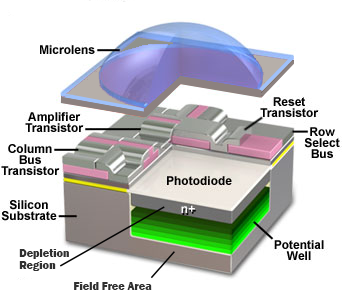
\includegraphics[height=2.9in]{Active Pixel Structure.png}
    \caption{Structure of a CMOS active pixel \cite{website:turchetta24}.}
    \label{fig:ActiveStructure}
\end{figure} 

\begin{itemize}[noitemsep]
    \item \textbf{Photodiode}: The photosensitive portion of the pixel;
    \item \textbf{Potential Well}: Storage location for photoelectrons;
    \item \textbf{Field Free Area}: Region of thermal equilibrium;
    \item \textbf{Depletion Region}: Area depleted of electrons and holes;
    \item \textbf{Three Support Transistors}: Amplifier Transistor, Column Bus Transistor, Reset Transistor; 
    \item \textbf{Busses}: Row Select Bus, Column Bus;
    \item \textbf{Microlens}: Focuses Light into the PPD.
\end{itemize}

I have identified each of the structures that will be useful in understanding the noise discussion that follows (the microlens arguably plays little if any role in noise generation, but I labelled it because, well, its big and dominates the image.). The most important of these structures is the photodiode.

\subsubsection{The Photo Diode}

The photodiode is the pixel's photosensitive area where the photoelectric effect takes place. In the 3T type imager, this is one of three forms of an \emph{N Well} photodiode. This structure had come to dominate the CMOS industry because of its low noise, low dark current, low lag, and high quantum efficiency properties. (I should mention here that these traits are in comparison to other, previous CMOS technologies, not in comparison to CCD technologies, which are still, in many ways, lower noise, lower dark current, and lower lag then CMOS. CMOS does, in most cases, surpass CCDs in quantum efficiency). 

In current CMOS imagers, largely utilizing a design called the 4T transistor, discussed in Section~\ref{sec:3T4T}, the earlier N Well photodiode has been replaced with the \emph{pinned photodiode} (PPD). The PPD has better performance and noise properties, and also directly allows for high speed shuttering \cite{teranishi15}. Invented in 1980 by Nobukazu Teranishi and others at NEC \cite{website:WikiAPS}, the development and refinement of this device was directly responsible for allowing the current generation of CMOS technology to approach parity with CCD technology. Interestingly, although the PPD is considered 'low noise' in comparison to other photodiode types such as the N-Well and PN Photodiode, the PPD is responsible for either introducing, or introducing increased quantities of,  several noise mechanisms, including \emph{kTC noise}, \emph{1/f noise}, and RTS Noise. 


The pinned photodiode structure is also responsible for the majority of the extreme effects exhibited by CMOS imagers in response to exposure to radiation; its \emph{transfer gate} construct is susceptible to high energy proton displacement damage. Also, the \emph{depletion region} which underlies it is susceptible both to manufacturing defects and radiation induced electron trap creation, a process which drastically increase the thermal generation of dark current.

A schematic of a PPD is shown in Figure~\ref{fig:PPDStructure}. The diagram shows the essential components of the PPD.

\begin{figure}[!t]
    \centering
        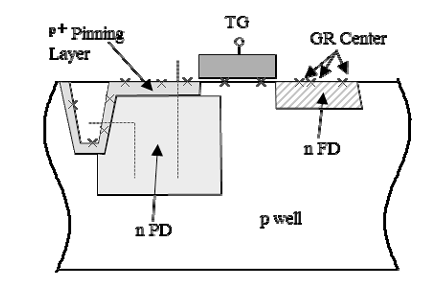
\includegraphics[height=2.0in]{PPD Structure.png}
    \caption{Structure of a Pinned Photodiode \cite{teranishi15}.}
    \label{fig:PPDStructure}
\end{figure} 

\begin{itemize}[noitemsep]
\item \textbf{nPD}: The active photodiode region of the PPD, where the photoelectric effect occurs;
\item \textbf{p Well}: The \emph{potential Well}, storage location during exposure for photoelectrons generated by the photodiode;
\item \textbf{GR}: The \emph{recombination-generation Center}, the location that supplies mobile charge carriers (electrons and electron holes) to the photodiode;
\item \textbf{\boldmath$p^+$ Pinning Layer}: The \emph{pinning layer}, which both protects the photodiode from thermally generated electrons from the GR region and creates a gradient allowing fast drift motion of signal electrons to the potential well. 
\item \textbf{TG}: The \emph{transfer gate}, the structure that regulates the flow of photoelectrons from the potential well to the floating diffusion region.
\item \textbf{nFD}: The \emph{floating diffusion region}, where electrons accumulate at readout, changing the voltage of the region, which is then read out by the \emph{sense node} as the pixel's final voltage.
\end{itemize}

This structure facilitates several useful mechanisms. It enables relatively low dark current; rapid discharge of signal electrons from the photodiode to the diffusion region, which reduces image lag, which in turns allows for the rapid electronic shuttering mentioned above.

\subsubsection{Three \& Four Transistor Design}
\label{sec:3T4T}

An essential part of active pixel design is the transistor layout. The \emph{three transistor design}, or \emph{3T APS}, is the original, most basic design.  In the 3T design, one transistor, the \emph{reset transistor}, is used to reset or precharge the photodiode. Another, the \emph{source follower transistor}, provides signal gain. And the third, the \emph{row}, or \emph{pixel select} transistor, provides the signal to each pixel to read out its voltage. A schematic of this design is presented in Figure~\ref{fig:3TSchematic}.

\begin{figure}[!t]
    \centering
        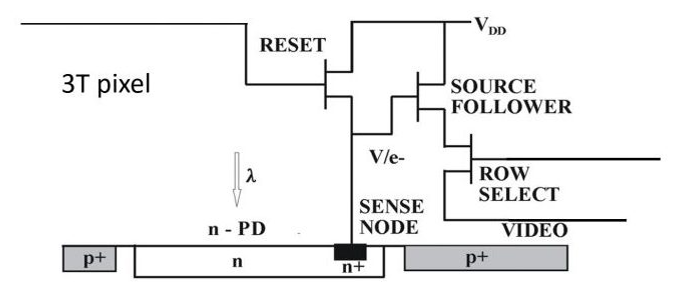
\includegraphics[height=2in]{3T CMOS Design.png}
    \caption{Functional Schematic of a 3T sensor's active pixel transistor design.\cite{website:EDN0120}.}
    \label{fig:3TSchematic}
\end{figure}


One of the major drawbacks of the 3T APS design concerns the reset transistor. When the reset transistor initializes the photodiode, a burst of noise, called '\emph{kTC noise}', is sent to the input node of the source follower transistor. Reset noise is of high magnitude, and reduces the signal-to-noise characteristics of the sensor considerably. For this reason, the architecture of the 3T has been evolved.

Current PPD CMOS sensors implement a technique called '\emph{correlated double sampling} (CDS)', which first measures the reset noise by itself, and then measures the reset noise combined with the signal. The noise is then subtracted from the combined signal. In order to do this, two changes were made. The first is the change from an N-Well photodiode to the pinned photodiode. The second is the addition of a fourth transistor to the active pixel structure, the '\emph{transfer transistor}', creating a \emph{4T APS CMOS} type sensor. This noise correction system also acts to reduce another type of CMOS noise, called 1/f noise, also referred to as \emph{amplifier noise}. 1/f noise is a form of low frequency noise, from which it gets its other name \emph{flicker noise}, so called because its frequency is low enough to be seen as flickering by the eye.

A direct result of the multi-transistor 3T/4T design is \emph{fixed pattern noise} (FPN). FPN is a result of manufacturing process inconsistencies leading to variations in the source follower transistor's gain in pixels across the sensor array. The result is a spatial noise pattern that is not mitigated by the CDS process. 

\begin{figure}[!b]
    \centering
        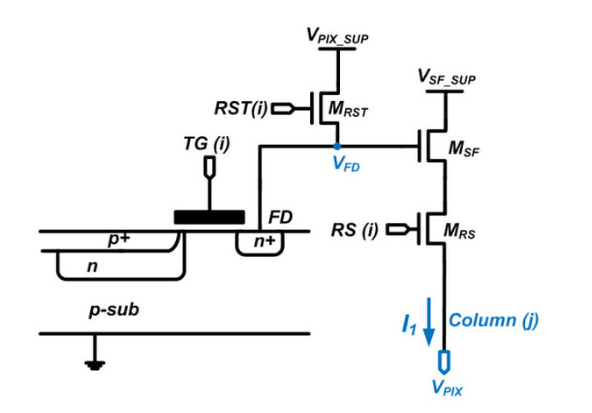
\includegraphics[height=2.0in]{APS Pixel Schematic.png}
    \caption{Functional Schematic of a 4T sensor's active pixel transistor design. \cite{xie19}.}
    \label{fig:PixelSchematic}
\end{figure}

\subsubsection{4T Active Pixel Functionality}

Figure~\ref{fig:PixelSchematic} shows a functional schematic of an active pixel. The labeling is as follows:

\begin{itemize}[noitemsep]
\item \textbf{FD}: Floating diffusion region
\item \textbf{TG}: Transfer gate and transfer transister;
\item \textbf{MRST}: Reset transistor
\item \textbf{MSF}: Source follower transistor (amplifier)
\item \textbf{MRS}: Row select transistor.
\item \textbf{Column}: Column bus Line
\end{itemize}

The area to the left of the transfer gate represents the pinned photo diode. The area under the photodiode represents the potential well. In abbreviated form, the pixel readout process proceeds as follows:

\begin{enumerate}[noitemsep]
\item Impinging photons are converted to electrons in the pinned photo diode.
\item Electrons are transferred and held in the potential well.
\item The transfer gate is signalled to open by the transfer gate transistor by the sequential readout of pixels at the end of the exposure, and electrons flow into the floating diffusion region.
\item The source follower transistor monitors the floating diffusion region's potential.
\item The floating diffusion region's final potential is transferred to the column bus line by the row select transistor.
\item The floating diffusion region is reset by the reset transistor.
\end{enumerate}

This is probably enough information about active pixel structure and functionality to understand the sources of noise related to CMOS pixels. Next up is sensor architecture and signal processing.

\subsection{CMOS Architecture and Functionality}


\begin{figure}[!b]
    \centering
        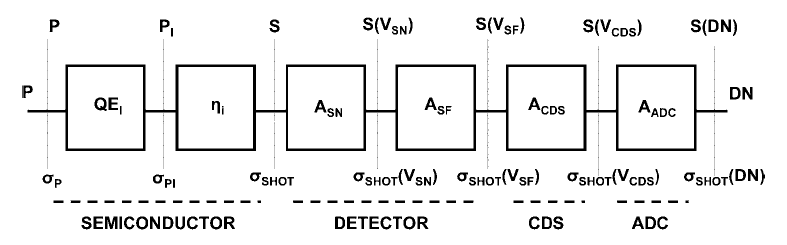
\includegraphics[height=1.7in]{CMOS Block Diagram.png}
    \caption{Block diagram for a typical CMOS imaging sensor, showing internal gain functions (values inside of blocks), signal parameters (values above blocks) and noise parameters (values below blocks) \cite{janesick}.}
    \label{fig:FuncSchematic}
\end{figure}

\subsubsection{CMOS Block Diagram}
\label{sec:transdiagram}

The easiest way to understand the functional architecture of a CMOS imaging sensor, and the flow of signal through it, is through the use of a \emph{functional block diagram}, sometimes also called a '\emph{readout chain}'. The block diagram also makes it easier to visualize the points in which shot noise is produced within that flow. A typical CMOS block diagram is shown in Figure~\ref{fig:FuncSchematic}. The following sections identify the various symbols on the block diagram.


\subsubsection{CMOS Transfer Functions}

The block diagram consists of a string of transfer functions, and each of these transfer functions are related to a physical structure, such as processing electronics, pixel structure, the semiconductor, transistors, etc. Transfer functions are essentially gain functions.

The following is a list of the represented transfer functions:

\begin{itemize}[noitemsep]
\item \textbf{\boldmath$QE_1$}: Quantum Efficiency;
\item \textbf{\boldmath$\eta_1$}: Quantum Yield Gain;
\item \textbf{\boldmath$A_{SN}$}: Sense Node Gain; 
\item \textbf{\boldmath$A_{SF}$}: Source Follower Gain;
\item \textbf{\boldmath$A_{CDS}$}: Correlated Double Sampling Gain;
\item \textbf{\boldmath$A_{ADC}$}: Analog to Digital Converter Gain.
\end{itemize}

Although some of these have been discussed previously, a few definitions are in order.

\paragraph{Quantum Yield Gain:} Essentially the number of electrons produced per photon. Whereas quantum efficiency indicates the likelihood of a sensor producing electrons from incident photons, quantum yield gain indicates the number of electrons produced per incident photon. For the purposes of this paper, $\eta_I = 1$.

\paragraph{Sense Node Gain:} The sense node region, which can be seen in Figure~\ref{fig:PixelSchematic}, is the structure where signal charge (electrons) are converted to working voltage. It is represented physically by the floating diffusion portion of the PPD (see Figure~\ref{fig:PPDStructure}).

\paragraph{Source Follower Gain:} Physically, the source follower is one of the transistors in a 3T/4T CMOS. It's job is to buffer (amplify) the voltage output of the sense node.

\paragraph{Analog to Digital Converter Gain}
The job of the \emph{analog-to-digital converter} is to take the voltage determined by the floating diffusion region, transferred through the column bus and sent to it across the row bus, and convert that voltage to digital numbers. More about the ADC in Section~\ref{sec:quant}.

\subsubsection{System Transfer Function}

At the left side of the diagram, \textbf{P} is the average number of incident photons per pixel. At the end of the diagram, \textbf{DN} is the average DN encoded for each pixel. By using block diagram algebra, the overall transfer function (total gain) of the CMOS is then:

$$\frac{S(DN)}{P}=QE_1 \cdot \eta_1 \cdot A_{SN} \cdot A_{SF} \cdot A_{CDS} \cdot A_{ADC}$$

\subsubsection{CMOS Camera Signals}

Along the top of the diagram are the camera signal parameters, indicating the various signals resulting from the previous signal being modified by the preceding transfer function. This is helpful to see at what point photons become electrons, electrons become a voltage measurement, and then when voltages become digital numbers (DN). The various camera signals are listed here:

\begin{itemize}[noitemsep]
\item \textbf{\boldmath$P$}: Incident Photons;
\item \textbf{\boldmath$P_1$}: Interacting Photons;
\item \textbf{\boldmath$S$}: Sense Node Electrons; 
\item \textbf{\boldmath$S(V_{SN})$}: Sense Node Voltage;
\item \textbf{\boldmath$S(V_{SF})$}: Source Follower Voltage;
\item \textbf{\boldmath$S(V_{CDS})$}: Correlated Double Sampling Voltage;
\item \textbf{\boldmath$S(DN)$}: Analog to Digital Converter Signal.
\end{itemize}

\subsubsection{CMOS Noise Parameters}
\label{sec:noiseparam}

Associated with each of these camera signals is an accompanying noise parameter. These parameters represent forms of shot noise, indicating that every transfer function adds shot noise to the signal. Note that transfer function shot noise is not the only form of noise inherent to CMOS imaging, and the block diagram is indicating only noise arising from the motion of particles, such as photon shot noise, and various forms of current shot noise, such as dark current shot noise, along with other minor quantities of shot noise introduced by transfer function components. For a modified version of this diagram indicating all forms of noise discussed in this paper, see Section~\ref{sec:combinednoise}.

\begin{itemize}[noitemsep]
\item \textbf{\boldmath$\sigma_{SHOT}(P)$}: Incident Photons;
\item \textbf{\boldmath$\sigma_{SHOT}(P_I)$}: Interacting Photons;
\item \textbf{\boldmath$\sigma_{SHOT}$}:  Sense Node Electrons; 
\item \textbf{\boldmath$\sigma_{SHOT}(V_{SN})$}: Sense Node Voltage;
\item \textbf{\boldmath$\sigma_{SHOT}(V_{SF})$}: Source Follower Voltage;
\item \textbf{\boldmath$\sigma_{SHOT}(V_{CDS})$}: Correlated Double Sampling Voltage;
\item \textbf{\boldmath$\sigma_{SHOT}(DN)$}: Analog to Digital Converter Signal.
\end{itemize}

With the discussion of structure and architecture out of the way, there remains one thing to discuss before proceeding to sources of CMOS imager noise, and that is how it is quantified.

\section{The Mathematical Analysis of Noise}

Before continuing on to discuss different noise sources and mechanisms, it is helpful to understand the math and notation used when discussing noise. This is going to be a very brief presentation, giving enough information to continue into the following sections. There are only a handful of essential mathematical tools to understand that are used in the analysis of imager noise. These are presented below.

Mathematically, noise phenomena is typically modeled as \emph{continuous random variables}, and noise waveforms are modeled as random processes. This is done because, in many cases, we do not specifically know what magnitude of noise is affecting the signal at any particular moment.

\subsection{Continuous Random Variables}
\label{sec:contvar}

Any continuous random variable is completely specified by its \emph{probability density function}:

$$\int_{-\infty}^{\infty} f_x(x) \,dx = 1$$

\noindent for

\vspace{-2mm}

$$f_x(x) \ge 0$$

\vspace{2mm}

\noindent From the probability density function, we can calculate the mean:

$$\bar{X} = \int_{-\infty}^{\infty} xf_x(x) \,dx$$

\vspace{2mm}

\noindent as well as the mean squared:

\vspace{-2mm}

$$\bar{X^2} = \int_{-\infty}^{\infty} x^2 f_x(x) \,dx$$

\vspace{2mm}

The mean squared represents the average power of some signal $X$. The square root of this is the RMS power of the signal. RMS power represents an equivalent signal with constant power that is equivalent to the average power of $X$.

The variance of $X$, then, is:

\vspace{-2mm}

$$ \sigma ^2 _X = \bar{X^2} - (\bar{X})^2$$

\vspace{2mm}

\noindent The variance of the signal $X$ is used in noise analysis as an estimate of noise power. The square root of the variance is $\sigma$, the standard deviation, which is used to express the quantity of noise resulting from a specific source. The sigma value, while representing the standard deviation of the noise component from the signal, can be read as the number of electrons of noise that are associated with a signal composed of some quantity of photoelectrons. As an example, for photon shot noise,
\vspace{-2mm}

$$ \sigma_{\text{PS}} = \sqrt{S} $$

\vspace{2mm}

\noindent which can be taken to indicate that, say, for a real signal of 100 photoelectrons produced by a light source, 10 photoelectrons of noise will be produced via the mechanism of photon shot noise.

\subsection{Noise Distribution Functions}

In the equations for the mean and the mean square given above, $f(x)$ represents a distribution of noise magnitudes. The two most common random variable functions used in noise analysis to model the magnitude distribution of noise are the Poisson distribution, used to model forms of shot noise (photon shot noise, dark current shot noise), and the Gaussian distribution, used to model almost everything else (1/f noise and thermal noise, for instance). 

\subsubsection{Poisson Distribution}

The Poisson distribution is a discrete probability distribution. It is given by the equation:

$$P(X=x) = f(x)=\frac{\lambda^x}{x!} \cdot e^{-\lambda}$$

\noindent for:

\vspace{-4mm}

$$x \ge 0$$

\noindent which can be read as the probability that $x$ events occur with $\lambda$ being the average rate of the occurrence of the events. 

The Poisson distribution has the following properties:

\vspace{-1mm}

$$ \text{Mean} = \mu = \lambda$$
$$ \text{Variance} = \sigma^2 = \lambda$$
$$ \text{Standard Deviation} = \sigma = \sqrt{\lambda}$$

\vspace{2mm}

\noindent Note that an important feature of the Poisson distribution is that its variance is equal to its mean. Use of the Poisson distribution to describe photon shot noise is discussed in Section~\ref{sec:psn}.

\subsubsection{Gaussian Distribution}

The Gaussian distribution, or normal distribution, is a continuous probability distribution. It has the form:

$$f(x) = \frac{1}{\sqrt{2 \pi \sigma^2_X}} \cdot e^{- \frac{(x-\bar{X})^2}{2 \sigma ^2_X}}$$

\noindent for:

\vspace{-4mm}

$$ -\infty < x < \infty $$

\vspace{2mm}
\noindent The variables here follow the discussion of Section~\ref{sec:contvar}. The Gaussian distribution has the following properties:

$$ \text{Mean} = \mu $$
$$ \text{Variance} = \sigma^2 $$
$$ \text{Standard Deviation} = \sigma $$

\subsection{Quadrature}

It should be noted that noise sources add their contributions in quadrature. If we have a classification of noise that contains noise from several sources, the total contribution from those sources would be:

$$ \sigma_{\text{CLASS}} = (\sigma^2_{\text{S1}} + \sigma^2_{\text{S2}} + \sigma^2_{\text{S3}} + \ldots )^{\frac{1}{2}}$$

\subsection{Signal-to-Noise Ratio}

Signal-to-noise analysis is the last topic to discuss here. SNR analysis is essential to determining an imager's performance, and is frequently a primary figure of merit in design and operation. The general notation for the signal-to-noise ratio is as follows:

$$ \left [ \frac{S}{N} \right ] _{\text{XX}} = \frac{S}{\sigma_{\text{SOURCE}}} $$ 

\vspace{2mm}

\noindent where 'xx' describes the situation under which the ratio is being calculated, and $ \sigma_{\text{SOURCE}} $ is the total of all noise source relative to the situation, added in quadrature.

For instance, if we are calculating the signal-to-noise ration of an imager under flat-field illumination, we would write:

$$ \left [ \frac{S}{N} \right ] _{\text{FF}} = \frac{S}{\sigma_{\text{TOTAL}}} $$ 

\vspace{2mm}

\noindent where $ \sigma_{\text{TOTAL}} $ is the total of all noise sources affecting the sensor added in quadrature.

Signal-to-noise can also be calculated for individual noise sources, or classifications of noise. If we wanted to know the contribution of read noise to the sensor's overall flat field noise profile, for instance, we would write:

$$ \left [ \frac{S}{N} \right ] _{\text{FF,READ}} = \frac{S}{\sigma_{\text{READ}}} $$ 

\vspace{2mm}
Signal-to-noise is discussed in Section~\ref{sec:SNR}.

\section{Types of CMOS Noise}
\label{sec:cmosnoise}

When photons strike a photosensitive detector and are processed by an imaging sensor, \emph{noise}, or \emph{signal variance} is produced. In this section, I'll discuss the various types of noise produced by CMOS sensors, where it originates, and methods of dealing with it.

\subsection{Classification of Noise}

It's helpful to understand the various ways in which noise is classified and referred to. Section~\ref{sec:classification}, started with the division of noise into \textbf{signal noise} and \textbf{sensor noise}, which is correct but rather limited. 

Next, sensor noise can be broken down into its \textbf{temporal} and \textbf{spatial} components. Temporal noise is the temporal variation in pixel output. Spatial noise is pattern noise that remains mostly fixed, varies across the sensor array, and is different from chip to chip. This is perhaps the most useful classification, because almost all of the noise handling techniques ('\emph{denoising}') that astronomers are familiar with, such as the application of dark frames, bias fields and flat fields, really only address the spatial components of noise, because the techniques for handling temporal noise are few and limited in their effect. (This is, however, a major topic of current research, with a few promising methodologies. See Section~\ref{sec:Mitigation}.) For this reason, the temporal component of image noise sets a fundamental limit on image sensor performance, particularly in low light applications \cite{tian99}. Sometimes the terms '\textbf{White Noise}' for the temporal component and '\textbf{Color Noise}' for the spatial component are used.

Another way to look at noise is how it relates to the signal itself. All shot noise, such as photon shot noise and dark current shot noise, goes as the square root of the signal. Fixed pattern noise increases proportionately to the signal. These are classified as '\textbf{Signal-Dependent Noise}'. All other forms of noise are not dependent on the signal, but may depend on other factors, as is the case with the thermal dependence of dark current. These other sources are '\textbf{Non-Signal Dependent noise}'. 

The following are the various types of noise, where they originate, and what can be done to mitigate them. Noise reduction is further discussed in Section~\ref{sec:Mitigation}.

\subsection{Photon Shot Noise (\boldmath $\sigma_{\text{P}}$)}
\label{sec:psn}

\subsubsection{Definition}

Photon shot noise is a form of temporal noise exhibited by particle phenomena, and one of several forms of CMOS noise that exhibits a Poisson distribution (see Section~\ref{sec:transfer}), all of which are collectively referred to \emph{signal shot noise}. Photon shot noise arises from the particle nature of light, just as electronic shot noise arises from the quantization of electrical charge.  

\subsubsection{Mechanism}

To understand the phenomena, consider a particle beam with a constant flux rate $\phi_p$. In time $t$, the average number of particles incident on a surface is $\phi_p \cdot t$. If each particle has the same probability of incidence, P(i), the number of incident particles obeys a Binomial Distribution. As the probability P(i) approaches 1, the binomial distribution approaches a Poisson distribution:

$$P_n(t)=\frac{(\phi_p \cdot t)^n}{n!} \cdot e^{-\phi_p \cdot t}$$

\vspace{-2mm}

\noindent where:

\begin{itemize}[noitemsep]
\item \textbf{\boldmath$n$} is the number of particles,
\item \textbf{\boldmath$\phi_p$} constant flux rate of particles,
\item \textbf{\boldmath$t$} is elapsed time, and
\item \textbf{\boldmath$P_n(t)$} is Probability of n incident particles in time $t$.
\end{itemize}

Because it is a Poisson distribution, it has the property that its variance is equal to its expectation value, such that:

$$E(n)=\sigma^2=\phi_p \cdot t$$

\noindent Therefore,

$$\sigma_{SHOT}=\sqrt{\phi_p \cdot t}$$

\vspace{0.4cm}

All shot noise phenomena originate in the fundamentally unpredictable nature of quantized processes, such as, in the case of photon shot noise, the nature of fluorescence. The randomness in direction and timing of photon emission from a fluorescent source leads to a beam of photons whose cross sectional density displays Poisson statistics. The way these photons spatially arrive at the detector then gives rise to Poisson variance, which is the noise associated purely with the interaction of photons with the sensor. In the block diagram, this is:

\vspace{0.2cm}

$$\sigma_P = \sqrt P$$

\vspace{2mm}

Note, however, that while photon shot noise is signal noise, there are many sources of shot noise that fall into the sensor noise classification. All are related, in one way or another, to the flow of electrons. Shot noise is essentially a \emph{particle} phenomena, and the flow of electrons obeys Poisson statistics in the same way that photons do. For more on other sources of shot noise, see Section~\ref{sec:noiseparam}.

\subsubsection{Mitigation} Because photon shot noise is inherent to the nature of light, and is temporal in nature, it cannot be eliminated. It can be reduced, however, by increasing exposure time or the intensity of the incident beam, because as P increases, $\sqrt P$ increases much more slowly.

\subsection{Dark Current (\boldmath $\sigma_{\text{D}}$)}

\subsubsection{Definition}

Dark current is charge generation in the absence of sensor illumination, and it is one of the first forms of noise in the readout chain. Under normal operational circumstances, dark current is one of the main sources of noise in CMOS sensors, is the noise source that effectively sets a minimal length of integration, and sets the base current level that the photo level must exceed to be detected. The mechanisms that generate dark current are all dependent on thermal processes within different regions of the PPD. 

\subsubsection{Mechanisms}

Dark current charge generation occurs in the PPD through a variety of mechanisms, and is then moved by a potential gradient through the transfer gate into the potential well. The mechanisms underlying dark current charge generation are:

\paragraph{Depletion Region Generation}
One of the primary sources of dark current generation occurs in the \emph{Depletion Region} of the PPD (see Figure~\ref{fig:ActiveStructure}). The depletion region is an area underlying the PPD structure that is devoid of electrons and holes, but contains traps. These traps participate in a process called '\emph{trap assisted carrier generation}', also called '\emph{hopping generation}', the efficiency of which increases with temperature increase \cite{janesick}.

\paragraph{Diffusion Dark Current}
Diffusion Dark Current starts in the \emph{Field Free Region}, a region of the area underlying the pixel structure that has a negligible electric field, is thermally stable, but is populated with charge carriers. The active pixel structure itself, however, does have a field, and electrons from this region diffuse into the potential well, a process whose efficiency again is increased with increasing temperature.

\paragraph{Dark Current Shot Noise (\boldmath $\sigma_{\text{D}}$)}
The combination of depleted area generation and diffusion dark current produces a steady flow of diffuse current which flows into the potential well. Above and beyond the undesired electrons it deposits in the potential well, which is a form of Gaussian noise, the current density is Poisson distributed and therefore has a form of shot noise associated with it, called \emph{Dark Current Shot Noise}, that occurs as it passes the potential well boundary. It is given by:

$$ \sigma_{\text{D}}=\sqrt (\text{N}_{\text{D}}) $$

\vspace{0.2cm}
\noindent where $\text{N}_{\text{D}}$  is the average number of dark current electrons generated in a given integration time.

\subsubsection{Mitigation}
\label{sec:DCMitigation}

The only way to reduce the effect of dark current is to cool the image sensor, which reduces the flow of thermal electrons to the potential well and thereby decreases noise from this source substantially. 

There is, however, persistent patterning to the production of the electrons generated by these mechanisms which varies from pixel to pixel but remains consistent over time. This fixed patterning is the spatial component of dark current, known as dark current fixed pattern poise (DFPN).  This patterning is a component, along with pixel fixed pattern noise (PFPN), column fixed pattern noise (CPFN), Dark Signal Non-Uniformity (DSNU) and Dark Signal Non-Uniformity (DSNU), of \emph{fixed pattern noise}, discussed below in Section~\ref{sec:FPN}. Further reduction of the effect of dark current, then, involves characterizing the sensor's fixed pattern noise and subtracting it off in post-acquisition processing).

\subsection{Transfer Noise (\boldmath $\sigma_{\text{CTI}}$)}
\label{sec:transfer}
\subsubsection{Definition}

Transfer noise is a form of temporal noise that results from the process of the incomplete transfer of charge from the potential well to the floating diffusion region through the transfer gate. It is a form of both shot noise and charge lag that is not corrected by the CDS system. There are two mechanisms that produce it, both relating to imperfections in pixel structure, known as '\emph{Charge Transfer Non-Idealities}'.  

\subsubsection{Mechanisms}

\paragraph{Potential Well Non-Ideality}
The first mechanism underlying transfer noise has to do with the fringing fields that are used to structure the shape of the potential well. It is frequently the case that due to variation in pixel structure resulting from the manufacturing process, the field is not applied consistently, and the resulting change of potential in the well causes electrons to cluster at the transfer gate. This leads to slower transfer (\emph{lag}), called \emph{Charge Transfer Inefficiency} (CTI). Further, some of these electrons diffuse back into the diffusion region (\emph{spill back lag}). This underlies the phenomena of \emph{image lag}. Sensors that exhibit substantial amounts of image lag most likely had issues during manufacture that may affect other performance parameters.

\paragraph{Transfer Gate Non-Ideality}
The second mechanism concerns the transfer gate itself. Again, because of the manufacturing process, the $\text{Si-SiO}_{\text{2}} $ area underlying the transfer gate frequently contains traps. Electrons flowing from the diffusion region to the potential well literally become trapped at the gate. Because this represents a current flow incident on the boundary of a region, it is also a form of spill back lag.

Spill back, because it is a form current flow, is a source of temporal shot noise, and is given by:

$$ \sigma_{\text{CTI}}=\sqrt (\text{CTI} \cdot \text{N}) $$

\vspace{2mm}

\noindent where CTI is a measured quantity determined by taking multiple sets of two consecutive readouts of large integration time, averaging each of the first exposures and then the second exposures, and determining the ratio between the two averages. This should be done during characterization to detect subtle manufacturing defects in any particular imager.

\subsubsection{Mitigation}

Transfer noise is temporal noise, and therefore falls into the classification of noise that can't really be dealt with directly but can potentially be dealt with during post acquisition processing with white noise routines (Section~\ref{sec:Mitigation}).

\subsection{Electronic Noise (\boldmath $\sigma_{\text{SF}}$)}

\subsubsection{Definition}

\emph{Electronic noise}, also called \emph{pixel source follower noise}, arises from several uncorrelated sources in the sensor package's readout circuitry (labelled as \emph{detector} in the block diagram), and has five components: kT/C Noise, MOS Transistor Thermal Noise, 1/f Noise, RTS Noise, and Leakage Current Shot Noise. Each are discussed below. One of these, kTC noise, is also produced in the APS structure by the firing of the reset transistor. 

Of these forms of noise, RTS noise and 1/f noise are of particular concern. Leakage current is generally negligible, but may become a more substantial noise source as radiation degrades the imager.

\subsubsection{Mechanisms}

\paragraph{Thermal Noise  (\boldmath $\sigma_{\text{TH}}$)} 

\emph{Thermal electronic noise} is a separate phenomena from dark signal. Thermal noise in this sense refers to noise generated by electrical components, resulting from fluctuation in the velocity of charge carriers in conductive material due to thermal excitation \cite{janesick}. It is generated in every resistive element and connection in a circuit. It is modeled similarly to the noise generated by current moving through a resistor, or current moving through a resitor/capacitor combination. 

Thermal noise takes two forms. The first, \emph{MOS transistor thermal noise}, is the noise generated by the flow of current through resistive channels in large area MOS transistors. Under normal operating conditions, MOS noise is negligible. 

The second, \emph{kTC noise}, is noise caused by a voltage fluctuation across a capacitive device resulting from the thermal noise generated by a resistive element connected to it. Thermally generated kTC noise is also, under normal operating conditions, negligible.

\paragraph{Sense Node Reset Noise (\boldmath $\sigma_{\text{RESET}}$)}

As discussed in Section~\ref{sec:3T4T}, the reset transistor in a 3T type sensor is a strong source of kTC noise, leading to the creation of the correlated double sampling system in the 4T design. Most of this noise is effectively cancelled by that system; the remaining portion becomes a component of source follower noise.

\paragraph{1/f Noise (\boldmath $\sigma_f$)}

The origin of 1/f noise, also called flicker, or amplifier noise, is not well understood, but is pervasive in electronic devices. It is most likely the result of Silicon Oxide contacting the substrate in the region of the diffusion area, creating electron traps that then capture and release electrons randomly. This manifests itself as low frequency noise. As CMOS technology has scaled, flicker noise has increased as a component of a sensor's noise profile. It is a form of low frequency noise that is visible to the eye. Flicker noise is manufacturing quality dependent, and can be a considerable component of the noise profile. 

\begin{figure}[!b]
    \centering
        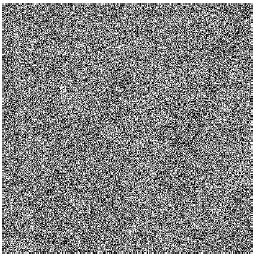
\includegraphics[height=1.7in]{Salt & Pepper Noise.png}
    \caption{RTS noise demo, 90\% noise level. \cite{fu19}.}
    \label{fig:RTSNoise}
\end{figure}

\paragraph{RTS Noise  (\boldmath $\sigma_{\text{RTS}}$)}
\label{sec:rtsnoise}

Perhaps one of the more obvious noise effects in CMOS imagers is Random Telegraph Signal Noise, or Salt and Pepper Noise (SAP) \cite{website:teldyne24}, also called '\emph{Impulse Noise}'. It is quite evident in dark frames, as shown in Figure~\ref{fig:RTSNoise}. Similar to 1/f noise, RTS has increased with the upscaling of CMOS imagers. SAP is a highly destructive form of noise, as it corrupts pixels by essentially overwriting their DN value with a zero or max DN, which makes it a difficult form of noise to correct. Also, SAP increases dramatically as a result of exposure to proton irradiation, the result of fundamental changes to the active pixel structure. 

\paragraph{Leakage Current Shot Noise (\boldmath $\sigma_{\text{LC}}$)}

Leakage current is undesired charge transport that occurs in either depleted regions or through insulators in all electronic devices; in CMOS imagers, they are effects the occur primarily in the sense node and transfer gate regions. They are the result of atomic-level stochastic errors inherent to the CMOS manufacturing processes. Fortunately, they are a minor contributor to the overall noise profile of any particular sensor; analysis shows that typical levels are around 0.001 $\text{e}^{\text{-}}$ and occurs between reset and sampling.

\paragraph{Pixel Source Follower Noise (\boldmath $\sigma_{\text{SF}}$)}

Collectively, these different forms of electronic noise are referred to as \text{source follower noise}. Whereas source follower noise in CCD imagers is domianted by flicker noise, RTS noise is the dominating factor in CMOS sensors. The overall composition of pixel source follower noise is then:

$$ \sigma_{\text{SF}} = (\sigma^2_{\text{TH}} + \sigma^2_f + \sigma^2_{\text{RTS}})^{\frac{1}{2}}$$

\vspace{2mm}

For bookkeeping purposes, leakage current shot noise and reset noise are added to the overall noise profile separately. See Section~\ref{sec:combinednoise}.

\subsubsection{Mitigation}
 
Like all forms of temporal noise, electronic noise is difficult, if not impossible to mitigate. RTS noise, in particular, is destructive, increases over time in exposure to radiation, and has been extremely difficult to address. Both temporal noise and RTS noise mitigation are the subject of Section~\ref{sec:Mitigation}.

\subsection{Fixed Pattern Noise (\boldmath $\sigma_{\text{FPN}}$)}
\label{sec:FPN}

\subsubsection{Definition}

Fixed pattern noise is spatial noise, that is, a type of noise that remains consistent in time across the array of any particular sensor but varies from chip to chip. It results primarily from variability in active pixel structure, called \emph{photo response non-uniformity (PRNU)}, resulting from CMOS manufacturing processes. It also has components resulting from gain differences in CMOS column amplifiers, called \emph{Column Level Gain Variation Noise}, and in individual pixel amplifying transistors, called \emph{Offset Spatial Variation Noise}. Collectively, these three components of fixed pattern noise are referred to as \emph{Light FPN}. Another component, \emph{Dark Signal Non-Uniformity}, results from the bias levels assigned to pixels to address the possibility of negative noise. And the final component is Dark Current Fixed Pattern Noise (DFPN), the persistent component of thermally generated dark current. These two components comprise \emph{Dark FPN}.

I should mention here that systematic defects in a sensor... such as dust motes, vignetting, shading, interference fringing, etc., all fall under the heading of FPN sources. 

\subsubsection{Mechanisms}

\paragraph{Photo Response Non-Uniformity (\boldmath $\sigma_{\text{PRNU}}$)}

PRNU originates primarily in two different regions of the pinned photo diode. One component is dominate at high signal levels, and is a result of pixel-to-pixel variations in quantum efficiency, pin voltage, and full-well capacity. The other component, which dominates at low signal levels, is a form of conversion gain mismatch, resulting from differences in the structure of the sense node junction, the transfer gate and the source follower. It is represented as follows:

$$ \sigma_{\text{PRNU}} = \text{P}_{\text{N}} \cdot \text{S}$$

\vspace{2mm}

\noindent where $\sigma_{\text{PRNU}}$ is the photo response non-uniformity in rms $\text{e}^{\text{-}}$ and $\text{P}_{\text{N}}$ is called the \emph{fixed pattern noise quality factor}, which is approximately 0.01 for both CCD and CMOS type sensors \cite{janesick}.

\paragraph{Column Fixed Pattern Noise (\boldmath $\sigma_{\text{CFNU}}$)}

Sometimes called \emph{Vertical Gain Mismatch}, this form of spatial noise results from inconsistency in the gain of CMOS column level amplifiers, and appears as easily perceived vertical lines in the image. Column level gain in CMOS is implemented with switched capacitor amplifiers, and hence gain differences are the result of capacitor mismatch, with typical mismatch values having a standard deviation on the order of 0.01\% \cite{boukhayma}.

\paragraph{Offset Spatial Variation Noise (\boldmath $\sigma_{\text{OFPN}}$)}

This form of noise primarily results from non-idealities in the structure of the active pixel's transfer gate and is a response to the switching of the transfer gate's voltage. Although most of this effect is cancelled by the CMOS CDS circuitry, theses structural issues can result in pixel gain variation even with CDS.

\paragraph{Dark Signal Non-Uniformity (\boldmath $\sigma_{\text{DSNU}}$)}

Dark signal non-uniformity is the result of applying bias to pixels to account for low signal levels whose noise may drive the pixel's reported voltage to negative values, resulting in negative DN numbers after ADC conversion. This patterning is what the creation of bias frames in traditional noise reduction technique is meant to address. It is important to note that this value is not constant across modes (gain settings, binning, etc.) and shows a weak temperature dependence, making the creation of bias frames for different mode combinations mandatory, and including different exposure lengths as a factor should be considered.

\paragraph{Dark Current Fixed Pattern Noise (\boldmath $\sigma_{\text{DFPN}}$)}
As discussed in Section~\ref{sec:DCMitigation}, Dark Signal Non-Uniformity is the persistent patterning resulting from an active pixel's generation of dark current. One measure of DSNU is given by:

\vspace{-4mm}

$$\sigma_{\text{DFPN}} = D \cdot D_N $$

\vspace{2mm}

\noindent where $D$ is the average dark current in electrons, and $D_N$ is the \emph{dark current FPN quality factor}, which varies between 10\% and 40\% for CMOS imagers.

\paragraph{Total Fixed Pattern Noise (\boldmath $\sigma_{\text{FPN}}$)}

For all sources of fixed pattern noise, we have:

$$ \sigma_{\text{FPN}} = (\sigma^2_{\text{PRNU}} + \sigma^2_{\text{CFNU}} + \sigma^2_{\text{OFPN}} + \sigma^2_{\text{DSNU}}+ \sigma^2_{\text{DFPN}})^{\frac{1}{2}}$$

\subsubsection{Mitigation}

Spatial noise is effectively mitigated, at least in ground-based applications, with traditional methods of astronomical image noise reduction that are utilized in post-acquisition processing, such as the application of dark frames, bias frames and flat fields. This is the topic of Section~\ref{sec:spatialnoisereduction}.

\subsection{Other Noise Sources}

\subsubsection{Definition}

This section contains two items: \emph{ADC quantizing noise} and \emph{system noise}. The second, system noise, is potentially composed of dozens of different sources, all dependent on the specific CMOS architecture and the manufacturing processes by which they were made. Whereas the first is well quantified and predictable, the second is stochastic and non-synchronous from frame-to-frame. \emph{Non-synchronous} in this usage means that noise levels alter significantly from one frame to the next under conditions of similar signal levels.

\subsubsection{Mechanisms}

\paragraph{ADC Quantizing Noise (\boldmath $\sigma_{\text{ADC}}$)}
\label{sec:quant}

Analog to digital quantizing (or quantization) noise is basically a rounding error between the input signal voltage and the digital number output. All quantization processes require rounding, and the difference between the desired voltage representation and the final converted DN is called the quantization error. Quantizing a sequence of numbers produces a series of quantization errors which manifest as quantization noise. 

As the effect of the conversion error is to create a variance in DN readings, this is almost a virtual form of noise (but quite real in effect), as it is not the result of errant electrons. 

To a certain extent, ADC noise is predictable. For an ideal ADC,

$$ \sigma_{\text{ADC(DN)}} = \left (\frac{1}{12} \right )^{\frac{1}{2}} \cdot AS = 0.2887S$$

\noindent In terms of virtual electrons, this amounts to:

$$ \sigma_{\text{ADC}} = 0.2887 \cdot K_{\text{ADC}} \cdot (\nicefrac{e^{\text{-}}}{\text{DN}}) \cdot S $$

\vspace{2mm}

\noindent Quantizing noise is dependent on the quantity $  K_{\text{ADC}} \cdot (\nicefrac{e^{\text{-}}}{\text{DN}}) $, called the \emph{ADC sensitivity}. ADC sensitivity is a quantity that can either be determined from the manufacturer's specification sheet information, or can be characterized with a powerful characterization tool known as a \emph{photon transfer curve} (PTC) (see Figure~\ref{fig:regimes} for an example of a photon transfer curve.) Sensors with higher ADC sensitivity values can produce noise ranging from being minimally apparent at the low end to overcoming the other components of read noise at the higher end. 

\paragraph{System Noise (\boldmath $\sigma_{\text{SYS}}$)}

The sources of system noise are almost too many to enumerate here, but a partial list would include \cite{janesick}:

\begin{itemize}[noitemsep]
\item Preamp noise;
\item Transient noise;
\item Settling and Ringing noise;
\item Ground Bounce noise;
\item Clock Phase Jitter noise;
\item Circuit Crosstalk noise;
\item Power Supply noise, resulting from unstable power supply voltage;
\item Oscillation noise.
\end{itemize}

System noise is temporal noise and considered to be dynamic, with levels changing from frame to frame (non-synchronous noise), and increasing significantly with each doubling of the frame rate. For long exposures, system noise is generally negligible. All forms of system noise are typically represented collectively as $\sigma_{\text{SYS}}$.

\subsubsection{Mitigation}

As a form of temporal noise, system noise is difficult to address. At longer exposure times, it is typically neglibgible, but White noise algorithms that address temporal noise can be applied. See Section~\ref{sec:temporalnoisereduction}.

\section{The Combined Effect of Noise}
\label{sec:combinednoise}

We can now get a somewhat comprehensive picture of the overall noise profile of a CMOS imaging sensor. Figure~\ref{fig:BlockFull} shows the block diagram from Section~\ref{sec:transdiagram}, Figure~\ref{fig:FuncSchematic}, modified to show all noise sources discussed in this paper. Each different source is indicated by '$\sigma_{\text{'SOURCE'}}$', at the location in the block diagram where the mechanism that produces the noise contaminates the desired signal. 

The sigma values are arranged into three classes. The types here are yet another classification scheme, commonly used in photon transfer curve characterization and analysis \cite{janesick}. This is the scheme I'll use in the discussion in this section. The main classes are:

\begin{figure}[!t]
    \centering
        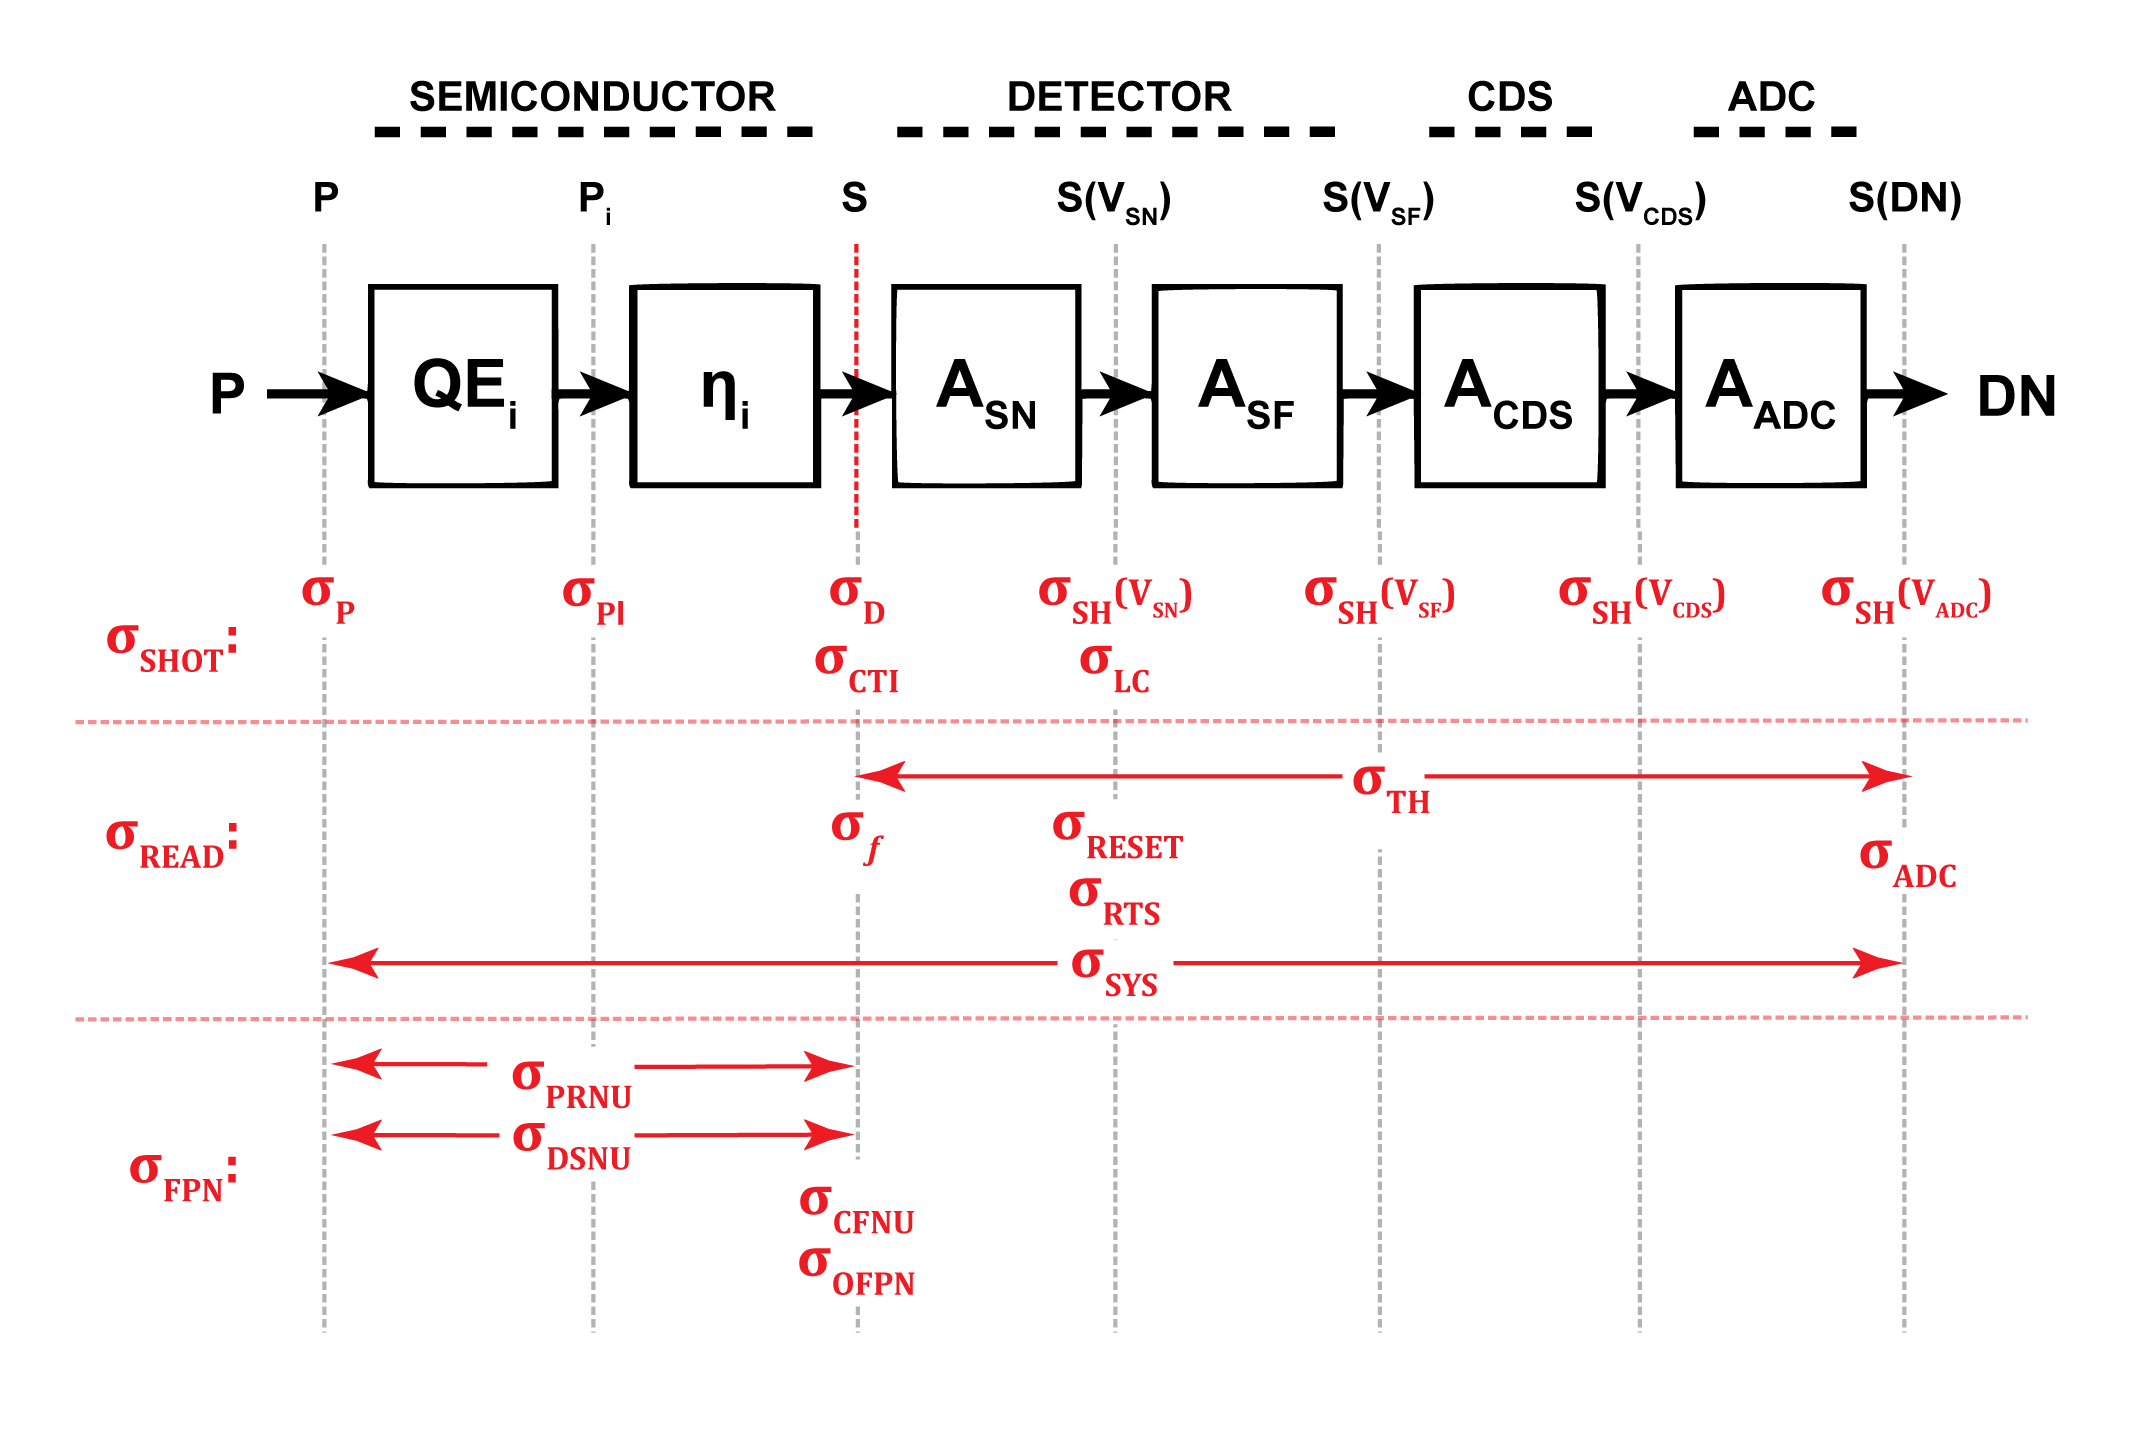
\includegraphics[height=3.75in]{assets/Block Diagram Full Noise.png}
    \caption{CMOS Imaging sensor block diagram, with all discussed noise sources included. At the top of the diagram is the physical structure that each transfer function is associated with. Under that are the average signal values at individual stages of signal processing, with 'P' representing photons, 'S' representing electrons, 'S(V)' representing various voltages, and 'S(DN)' representing digital numbers. Under this are the transfer, or gain functions as defined in Section~\ref{sec:transdiagram}. Under this are the noise sources discussed in this paper, grouped into three classes (Shot, Read, and FPN), with their horizontal positioning indicating at what stage in the signal process chain that they combine with the signal. \cite{janesick}.}
    \label{fig:BlockFull}
\end{figure}

\begin{itemize}[noitemsep]
\item Shot Noise (\boldmath $\sigma_{\text{P}}$): Both photon and current signal shot;
\item Read Noise (\boldmath $\sigma_{\text{READ}}$): Temporal noise originating in the detector, CDS and ADC;
\item FPN Noise (\boldmath $\sigma_{\text{FPN}}$): Spatial noise originating in the active pixel structure;;
\end{itemize}

Next, we'll write out the components of the noise and the equations of their contributions to the sensor's SNR for each of these three classes.

\subsection{Noise Equations}

Writing out the noise equations can be a little unwieldy because of the number of noise sources, but it's good to understand the components of each  of these three noise classes, especially when evaluating the contributions of each component to overall noise. 

Also, because one of the most important measures of image quality is the sensor's Signal-to-Noise ratio (SNR), its helpful to write out the SNR contributions from each class as well. The SNR equations here apply to uniform flat-field illumination.

\subsubsection{Shot Noise Equation}

Combining shot noise sources, we have:

$$ \sigma_{\text{SHOT}} = \sqrt{  \left ( (\sigma^2_{\text{P}} + \sigma^2_{\text{PI}} + \sigma^2_{\text{D}} + \sigma^2_{{\text{SH(V}_{{\text{SN}}})}} + \sigma^2_{{\text{SH(V}_{{\text{SF}}})}}+\sigma^2_{{\text{SH(V}_{{\text{CDS}}})}}+\sigma^2_{{\text{SH(V}_{{\text{ADC}}})}} )+  (\sigma^2_{\text{CTI}} + \sigma^2_{\text{LC}}) \right )^{\frac{1}{2}} }     $$

\paragraph{Shot Noise SNR Contribution}

Shot noise increases as illumination level increases, but signal also increases. Because the signal increases much faster than the shot noise, which is modeled as $\sigma_{\text{SHOT}} = \sqrt{S}$, shot noise SNR generally improves proportionally as illumination levels increase. The SNR within the shot noise class is given by:

$$ \text{SNR(SHOT)} = \left [ \frac{S}{N} \right ] _ {FF} = \frac{S}{\sigma_{\text{SHOT}}} = \frac{S}{S^{\frac{1}{2}}} = S^{\frac{1}{2}}$$

This indicates that the SNR from shot noise sources increases by the square root of the signal, which is a line with a slope of 1/2 on a log-log plot.

\subsubsection{Read Noise Equation}

Combining all read noise sources gives us::

$$ \sigma_{\text{READ}} = \sqrt{  \left ( (\sigma^2_{\text{TH}} + \sigma^2_{\text{RESET}} + \sigma^2_{\text{RTS}} + \sigma^2_f) + ( \sigma^2_{\text{ADC}} + \sigma^2_{\text{SYS}}) \right )^{\frac{1}{2}} }     $$

\paragraph{Read Noise SNR}

Read noise from all sources is independent of the input Signal. The read noise SNR is given by:

$$ \text{SNR(SHOT)} = \left [ \frac{S}{N} \right ] _ {FF} = \frac{S}{\sigma_{\text{READ}}} $$

This indicates that the SNR from read noise sources is proportional to the signal, which is a line with a slope of 1 on a log-log plot.

\vspace{2mm}

\subsubsection{Fixed Pattern Noise Equation}

Combining all fixed pattern noise sources gives us:

$$ \sigma_{\text{FPN}} = \sqrt{  \left ( \sigma^2_{\text{PRNU}} + \sigma^2_{\text{DSNU}} + \sigma^2_{\text{CFNU}} + \sigma^2_{\text{DFPN}} + \sigma^2_{\text{OFPN}} \right )^{\frac{1}{2}} }     $$

\paragraph{Fixed Pattern Noise SNR}

FPN noise increases proportionally to signal. The fixed pattern SNR is given by:

$$ \text{SNR(FPN)} = \left [ \frac{S}{N} \right ] _ {FF} = \frac{S}{\sigma_{\text{FPN}}} = \frac{S}{P_N \cdot S} = \frac{1}{P_N} $$

\vspace{2mm}

This indicates that the SNR from fixed pattern sources is independent of signal, which is a line with a slope of 0.

\subsubsection{Combined SNR From All Sources}

Combining the SNR equations, we can get the overall sensor SNR under condition of flat-field illumination:

$$ \text{SNR(TOTAL)} = \left [ \frac{S}{N} \right ] _ {FF} = \frac{S}{\sigma_{\text{TOTAL}}} =  \frac{S}{\left [ \sigma^2_{READ} + S^2 + (P_N \cdot S)^2 \right ]^ \frac{1}{2}} $$

\subsubsection{Summary of SNR Slopes}

For convenience, these are the log-log plot slopes of the \emph{SNR} curves in the different regimes:

\begin{itemize}[noitemsep]
    \item \textbf{Read Noise Regime}: $m=1$
    \item \textbf{Shot Noise Regime}: $m=\nicefrac{1}{2}$
    \item \textbf{FPN Regime}: $m=0$
    \item \textbf{Full Well Regime}: $m=\infty$
\end{itemize}

\subsection{Noise Regimes}

The way noise behaves in a CMOS sensor depends strongly on illumination level. Figure~\ref{fig:regimes}, from \emph{Janesick} \cite{janesick}, shows four distinct regions in an ideal noise versus signal log-log plot. This type of plot is an example of a photon transfer curve. It is produced by a relatively simple laboratory characterization procedure, but produces a wide range of characterization results. For instance, through PTC analysis one can determine full well capacity, total shot noise contribution, total read noise contribution, ADC sensitivity, linearity, total fixed pattern noise contribution, and quite a few more quantities of interest.


\begin{figure}[!t]
    \centering
        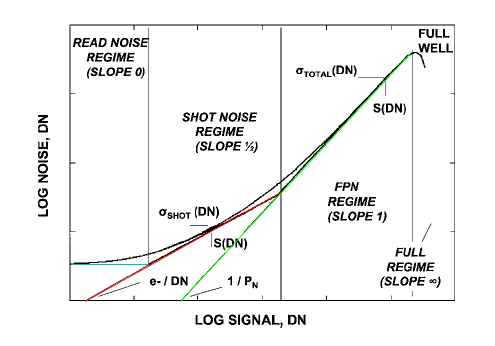
\includegraphics[height=3.0in]{Noise Regimes.png}
    \caption{Ideal signal versus noise photon transfer curve, showing the four signal regimes. \cite{janesick}.}
    \label{fig:regimes}
\end{figure}

\subsubsection{Description}

The plot shows RMS noise versus average input signal (essentially a representation of exposure time). At the left end of the x-axis, zero represents no input signal, such as in the situation of taking a dark frame. Signal in this regime is fully dominated by sources of read noise, represented by the blue horizontal line. The red angled line beneath it represents photon shot noise. As illumination level increases, the point where photon shot noise exceeds read noise marks the start of the shot noise regime, where the noise profile is dominated by shot noise, of which photon noise is proportionally the largest contributor. The characteristic 1/2 slope of shot noise is easily seen. Underneath the red line is a green line, representing fixed pattern noise. The point at which FPN exceeds photon shot noise marks the start of the FPN regime, where fixed pattern noise dominates the noise profile. 

The fourth region begins as pixels begin to hit their full well capacity. There is a rapid dropoff in noise as saturation is reached, although some CMOS types will show a continuing increase in FPN. This dropoff point is the way in which one characterization value, the full well value, can be determined from the PTC curve.

\subsubsection{Summary of Signal vs Noise Slopes}

Again, for convenience, and because they are similar enough to cause confusion, these are the slopes of the \emph{signal} curve in the different regimes:

\begin{itemize}[noitemsep]
    \item \textbf{Read Noise Regime}: $m=0$
    \item \textbf{Shot Noise Regime}: $m=\nicefrac{1}{2}$
    \item \textbf{FPN Regime}: $m=1$
    \item \textbf{Full Well Regime}: $m=\infty$
\end{itemize}

\subsubsection{Read Noise Regime}

The dominate noise sources in the read noise regime are RTS noise, which in essence sets the noise floor in this regime, flicker noise, and thermal noise, all of which typically sum to approximately 5 $\text{e}^{\text{-}}$ RMS. Other read noise sources are considered negligble, except in certain cases. For instance, in CMOS sensors with rolling shutter (RS) architecture, source follower reset noise is not entirely cancelled by the CDS system. The total amount of reset noise in a RS CMOS imager is dependent on the sense node gain, marked in the block diagram by $\text{A}_{\text{SN}}$. Typical state-of-the-art sense node gains are around $\text{50 } \nicefrac{\mu V}{\text{e}^{\text{-}}} $. At this gain, the sense node will be generating approximately 24 $\text{e}^{\text{-}}$ RMS, making it, for these sensors, the dominate form of read noise.

In terms of the noise sources discussed, then, we can rank them for the read noise regime as follows. For global shutter CMOS imagers:

$$ \sigma_{\text{RTS}} > \sigma_f > \sigma_{\text{RESET}} > \sigma_{\text{TH}} \gg \sigma_{\text{SYS}} > \sigma_{\text{ADC}}$$

\vspace{2mm}

For rolling shutter CMOS imagers:

$$ \sigma_{\text{RESET}} \gg \sigma_{\text{RTS}} > \sigma_f > \sigma_{\text{TH}} \gg \sigma_{\text{SYS}} > \sigma_{\text{ADC}}$$

\vspace{2mm}

An important note here concerns ADC quantizing noise. As discussed in Section~\ref{sec:quant}, the degree of ADC quantizing noise is dependent on the particular ADC's sensitivity value, expressed in electrons per DN. Lower is better. ADC sensitivity values can range between 2 and 100 electrons per DN. Whereas manufacturers rarely list the sensitivity of the ADC, they sometimes will list the ADC bit value. In general, the higher the bit level, the lower the quantization noise. For higher sensitivities and/or lower ADC bit values, ADC noise can dominate the noise floor, producing greater amounts of noise than either reset or RTC sources. This makes it imperative to include determining the ADC sensitivity during characterization.

\subsubsection{Shot Noise Regime}

In the shot noise regime, photon shot noise is by far the dominate noise source. Reducing sources of FPN in the fixed pattern noise regime to below the photon shot noise level effectively sets the noise floor to photon shot noise across a wide range of signal values, and the image produced in those signal ranges is then considered to be \emph{photon shot limited}. This is in practice the best noise reduction possible. 

Of the other effects that generate shot noise, the next predominate source is dark current shot noise, the temporal component of dark current. The temporal component of dark current is not its major component, however, as the spatial component, dark current fixed pattern noise, is by order of magnitude some 10-40 times greater. Dark current shot noise is really only of concern in higher temperature operation, as it is thermally generated and cooling the camera reduces dark current shot noise substantially. The DFPN component is effectively removed by flat-fielding. 

Leakage current shot noise is an interesting phenomena in that it inversely scales with the \emph{technology node size} of the sensor node. As APS technology evolves to produce smaller and smaller pixel sizes, the sense node technology node size decreases, and the leakage current value increases. The cutoff on node size is roughly 300nm (note that this does not refer to the actual size of a physical structure, but indicates the manufacturing process that creates the physical structure). At this point, leakage current shot noise is negligible, at about 0.001 e- RMS. As this size begins to decrease, the noise begins to increase rapidly by orders of magnitude, and leakage current shot noise can become the dominant form of shot noise.

Of the remaining forms of shot noise, the only other source that can be potentially of consequence is charge transfer non-ideality shot noise. This is largely dependent on the manufacturing process behind any particular CMOS imager. Typically it is negligible, but CTI should be determined in characterization to insure that it is. 

With these points in mind, we can rank shot noise sources as follows. The assumption here is that the camera is cooled, the sensor in question has a sense node created with 300nm or greater manufacturing technology, and that the sensor was not manufactured in a way that CTI characterization indicates that it has a high CTI factor.

$$ \sigma^2_{\text{P}} \gg \sigma^2_{\text{D}} \gg \sigma^2_{\text{LC}} > \sigma^2_{\text{CTI}} $$

$$ \sigma^2_{\text{P}} \gg \sigma^2_{\text{D}} >  (\sigma^2_{\text{SH(V}_{\text{SN}})} + \sigma^2_{\text{SH(V}_{\text{SP}})} + \sigma^2_{\text{SH(V}_{\text{CDS}})} + \sigma^2_{\text{SH(V}_{\text{ADC}})}) $$

\subsubsection{FPN Regime}

Because fixed pattern noise is proportional to the signal, it dominates all other noise sources in the fixed pattern regime. It is noise from a variety of sources, ranging from pixel-to-pixel gain variations, dark current fixed patterning, and column amplifier gain differences, to dust specks and interference fringing from glass sensor cover plates (sensor defects), to the applied pixel bias. It is also the most manageable form of noise, as it can be almost completely removed through careful use of flat-fielding. The typical FPN for a CMOS imager is about 1\% of the signal, far exceeding both the total read noise and the total shot noise noise of a sensor.

In terms of the contributions of individual sources, we can rank as follows:

$$ \sigma_{\text{PRNU}} > \sigma^2_{\text{DFPN}} \gg \sigma^2_{\text{CFNU}} > \sigma^2_{\text{DSNU}} > \sigma^2_{\text{OFPN}}$$

\vspace{2mm}

The defects component of fixed pattern noise is not included here, because defects result from unexpected mistakes in the manufacturing process and can vary greatly in effect. In certain cases, this type of defect can have huge implications for FPN. For instance, a slight misalignment in the parallel-plane geometry between the sensor's surface and the optical window of the camera can result in interference fringing, which can drive the noise percentage from FPN sources to as high as 10\% of the signal. 

\subsubsection{Full Well Regime}

In most CMOS sensors, noise modulation decreases just as pixels near full well, causing a rapid drop in noise on the photon transfer curve immediately before pixel saturation. 

In some CMOS structures, however, as pixels begin to fill, approaching the full-well point, some columns in the array may have all pixels reach full-well before others. This creates a type of column noise that results in the total FPN \emph{increasing} rapidly just before the sensor hits saturation. Shot noise still decreases, with the overall effect being an abrupt flattening of the curve.  

Determining which of the two behaviors occurs in any particular CMOS imager is a matter of looking at the nature of the change on the photon transfer curve. Either way, the \emph{point} at which the curve deviates significantly from the straight line that characterizes the fixed pattern noise regime sets the full-well capacity of the sensor. 

% ----------------------------------------------------------
% - Notes
% - Noise comparison Graphs:  p187, 191 Jane
% - ADC Quantizing Noise: p181 Jane

\subsection{Signal-To-Noise}
\label{sec:SNR}

\subsubsection{Sensor Signal-to-Noise}

In the same way that plotting noise versus signal gives us insight into which noise sources dominate in different signal regimes, we can determine when a sensor has its best signal to noise behavior by plotting signal-to-noise ratio versus noise. Such a plot is shown in Figure~\ref{fig:SNRregimes}. 



The figure shows two plots. The one on the left is a typical photon transfer curve for an imaging sensor illuminated with flat-field light. The one on the right is a corresponding signal-to-noise ratio versus signal plot. The plots have the same x-axis values, so that they can be easily matched. I have highlighted the regimes in Janesick's plot so that their boundaries are easier to see. I have also added a horizontal dotted blue line at a SNR value of ten, generally considered to be the cut off under which an image is deemed unacceptably noisy. 

One of the things that can be gleaned from this plot is that, for a fixed pattern noise quality factor of $ {P}_{\text{N}} = 0.02 $, the highest signal to noise ratio possible is 50:1, and this occurs in the signal range between 20,000 and 300,000 electrons per pixel. We can also determine the signal level cutoff for acceptable noise, which occurs at 100 electrons per pixel.

The usefulness of the SNR plot, besides its easy to use eyeballing of appropriate signal ranges, is that it allows us to determine the signal-to-noise ratio for \emph{any} signal level, for any sensor that has been characterized using photon transfer curve methodologies, from which appropriate exposure times can be calculated to achieve desired imager performance. 

\subsubsection{Image Signal-to-Noise}

\begin{figure}[!t]
    \centering
        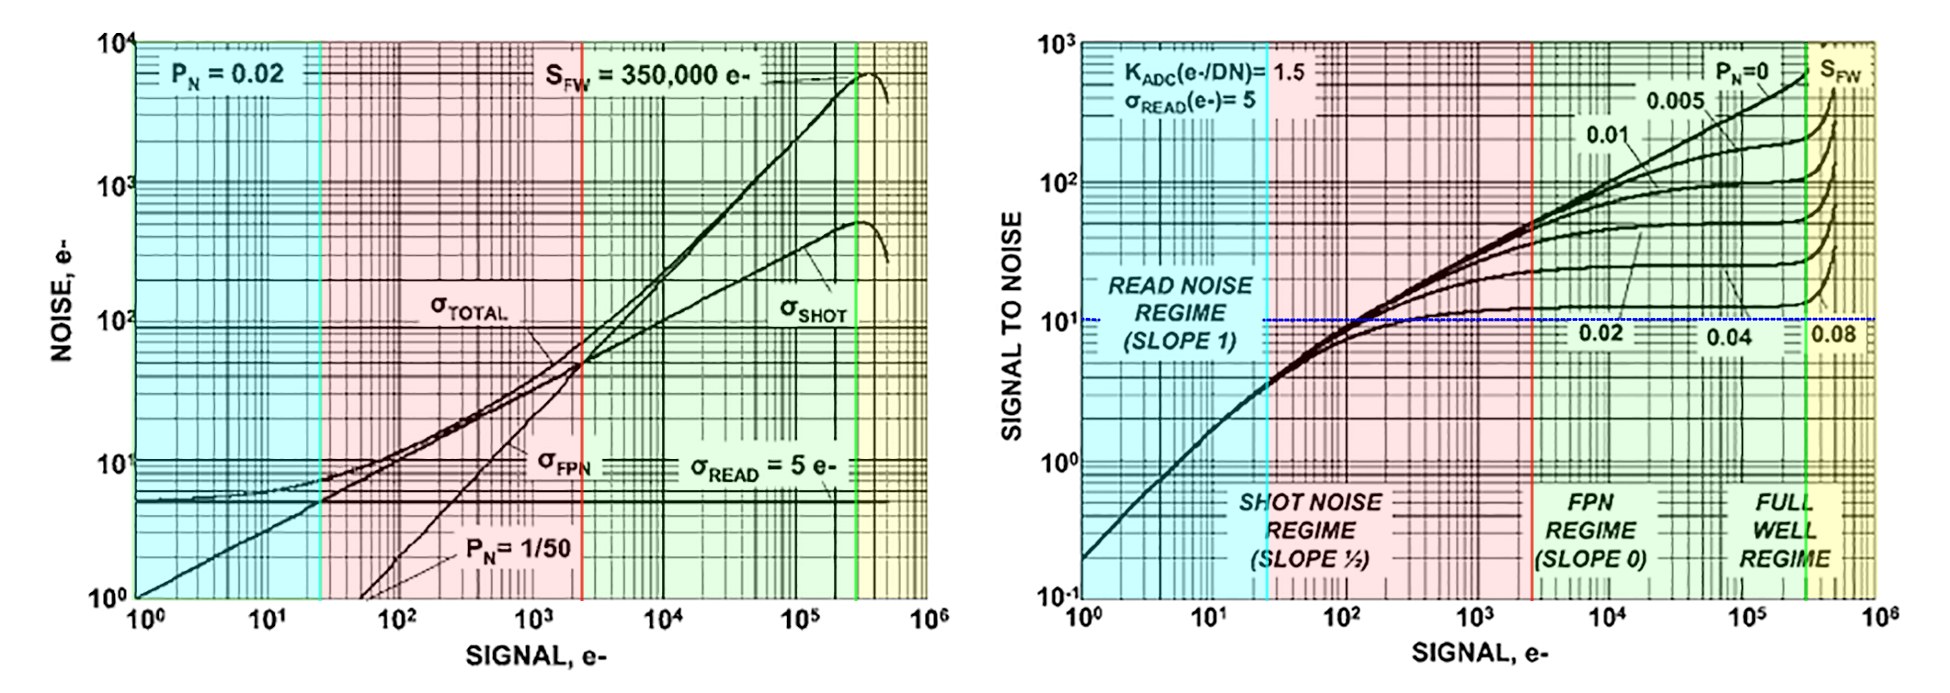
\includegraphics[height=2.31in]{SNR Plot 2 Double.png}
    \caption{A photon transfer curve (left) and its corresponding SNR plot (right) for an imaging sensor under flat-field illumination. Several quantities are indicated on the plots. On the PTC plot, $P_{\text{N}} = 0.02$ is the sensor's fixed pattern noise quality factor. $\text{S}_{\text{FW}} = 350,000 \text{e}^{\text{-}}$ is the sensor's full well capacity. The sigma value for read noise is given, and the lines are identified by the sigma values they represent. On the SNR plot, $\text{K}_{\text{ADC}}$ is the ADC sensitivity factor in electrons per DN, and the read noise is given as 5 electrons RMS. Each curve represents the sensor's SNR response to different levels of fixed pattern noise, with $0.02$ matching the PTC plot on the left.   \cite{janesick}.}
    \label{fig:SNRregimes}
\end{figure}


Images can be analyzed in this way as well. Instead of taking a photon transfer curve for a sensor, a variant type of PTC, called a \emph{modulation photon transfer curve}, is performed on the image data itself. 

The general signal-to-noise expression for an image is:

$$ \left [ \frac{\text{S}}{\text{N}} \right ] _{\text{I}}  = \frac{M_{\text{I}} \cdot S_{\text{I}}}{\sigma_{\text{I,TOTAL}}} $$

\noindent where $ M_{\text{I}}$ is the image modulation constant, which varies with the image contrast and is obtained from the modulation photon transfer curve. $ S_{\text{I}} $ is the signal level of the image, and $ \sigma_{\text{I,TOTAL}} $ is the total image noise, also obtained from the modulation PTC.

The important thing about this is that there is an important relationship between the image signal-to-noise and the sensor's flat-field signal-to-noise:

$$ \left [ \frac{\text{S}}{\text{N}} \right ] _{\text{I}}  = M_{\text{I}} \cdot \left [ \frac{\text{S}}{\text{N}} \right ]_{\text{FF}} $$

What we get from this is that, if we optimize the sensor's flat field signal-to-noise performance, we produce the highest signal-to-noise ratio for the images it creates. It also tells us, however, that  the image SNR will allows be smaller than the sensor's flat-field SNR by a factor of $ M_{\text{I}}$.

\section{Radiation and Noise}
\label{sec:RADeffects}

It is known that exposure to radiation causes changes to the noise profile of a CMOS sensor. Knowledge of these changes is essential to planning a strategy for mitigating the effects of a noise profile which is going to change substantially over the course of a mission. It is also essential in shaping the selection of characterization tests, so as to best understand those parameters and performance factors that are likely to change.. 

\subsection{Gamma Exposure} 

In a study by Feng, Wang, et. al. \cite{feng23}, CMOS sensors were exposed to gamma radiation produced by \textsuperscript{60}Co. Dark current was found to begin increasing almost immediately, with significant increases starting at 75 kRAD. It was found that exposure to 100 kRAD degraded CMOS MTF significantly, reducing camera resolution and increasing pixel to pixel crosstalk. Full well capacity was shown to begin dropping rapidly at around this level as well. At higher levels of exposure, spectral response began to drop rapidly. This behavior is important for our purposes, as the interaction of charged particles and aluminum shielding produces gamma radiation via Bremsstrahlung.

\subsection{The JANUS Camera}

Perhaps the most relevant reference to radiation degradation in space-based CMOS imagers comes from the JUpiter ICy moons Explorer (JUICE) mission, launched in April of 2023 by ESA to study  Ganymede, Callisto, and Europa. The science camera, JANUS, designed to operate between 400nm and 1000nm, is composed of a single CMOS APS imager, manufactured by e2v Technologies. As part of the JANUS team's characterization process, they studied the effect of proton and gamma radiation exposure on the e2v imager.

The most important result of their work concerned RTS noise \cite{winstone15}. In the initial sensor examination, the number of pixels found to exhibit repetitive RTS behavior was found to be 86,770, or 2.9\% of the total. They then exposed the sensor to irradiation with $\text{2.0} \times \text{10}^{\text{10}} $ 74 MeV protons per square centimeter over a period of time designed to mimic the projected mission TID, a quantity well within the range of expected energetic proton exposure in HEO orbits. It was found that the post exposure count of RTS affected pixels had increased to 1,209,600, or 40\% of the total array.

The JANUS team also examined the effect of proton irradiation on dark current \cite{soman15}. After the same exposure as in the RTS experiment, it was found that approximately 25\% of the sensor's pixels began exhibiting 'hot pixel' dark current levels of over 1000 $\text{e}^{\text{-1}}$. The same study found that transfer gate image lag increased by 2.5\%.

Another interesting result from the JANUS radiation studies concerns operational effects during irradiation, as opposed to long term degradation post irradiation \cite{soman16}. In this case, the source was 6.5 kRAD(Si) per hour from a \textsuperscript{60}Co source. It was found that the dark noise floor, initially at a mean across the ROI of 4500 DN, jumped immediately to a level of 9650 DN as soon as irradiation was started. This study also found a general 100\%+ increase in per-pixel read noise after exposure.

\subsection{Damage Mechanisms}

Given the dearth of information on the effects of space radiation on CMOS structure and function, the entire realm of potential long term radiation effects, as well as operational affects during exposure, are not well understood. However, the JANUS results do provide some insight.

The primary mechanism by which proton radiation damages CMOS sensors is through the high energy proton interaction with silicon. A proton striking the substrate can cause displacement damage, creating lattice defects that can act as traps for electrons, increasing thermal dark current noise. 

Irradiation also affects responsivity, saturation voltage and linear drift. This is linked to structural changes in the reset transistor and the transfer gate caused by by both gamma and proton irradiation. The fundamental cause for this behavior appears to be a flat band voltage shift of between 1.1 and 1.6 mV per kRAD resulting from trapped positive charge in the transfer gate.

From these results, we can also extrapolate that other noise mechanisms related to the same active pixel structures may well increase. Leakage current shot noise, for instance, is a noise mechanism tightly tied to the transfer gate. Charge Transfer Inefficiency generated noise, another transfer gate related noise mechanism linked to image lag, may also be affected.

And, perhaps, more troublesome is the increase in hot pixels following proton irradiation. This will affect both dark signal non-uniformity and fixed pattern noise in general, slowly degrading the performance of the library of calibration frames created during characterization (see Section~\ref{sec:spatialnoisereduction}).

\section{Noise Reduction}
\label{sec:Mitigation}

\subsection{Introduction}

There are fundamentally only two ways to reduce a CMOS imaging sensor's noise: by modifying the sensor's electronics, and by post acquisition processing, sometimes referred to as \emph{denoising}. Reduction of the spatial component of noise is fairly straightforward and effective; reduction of temporal noise generated by the CMOS structure and circuitry is far more difficult and an active subject of investigation. Each generation of CMOS technologies pushes the noise floor lower, but nature assures, primarily through photon and current signal shot noise, that noise will never entirely be defeated.

Since we have no control over the design of the sensors we use, modifying the sensor's electronics is not an option. That leaves us with post-acquisition processing. 

\subsubsection{Spatial Noise}

Removing spatial noise from an image is something that every observing astronomer is likely familiar with. It involves the acquisition of specialized exposure frames, called \emph{calibration images}, or \emph{calibration frames}, which are then used in a post acquisition process called \emph{data reduction}, or \emph{image calibration}. The purpose of traditional data reduction is to remove artifacts introduced into the image by persistent irregularities in the sensor or optics of the camera and to remove non-variant sources of noise introduced by the sensor's photoelectron generation process and signal processing circuitry. This is the topic of Section~\ref{sec:spatialnoisereduction} below.

There is an important caveat here. \emph{It should be noted that in space-based applications, where cameras may not have physical shutters or illumination by external light sources, these traditional methods, which usually require the on-the fly generation of various types of data-reduction fields, become more complicated.} In this case, substantial effort must be taken to generate libraries of various reduction frames, for each sensor, to be used during the mission. Even with this preparation, however, \emph{sensor degradation due to radiation exposure will slowly render even these frames less effective over the mission's duration}.

\subsubsection{Temporal Noise}

Removing temporal noise is a far more difficult endeavor. Removing spatial noise is like target practice with a bottle sitting on a wall; removing temporal noise is like using a blunderbuss to hit a bunch of flying bottles that wink in and out of existence, without blowing holes in everything else. 

Temporal noise has two important characteristics that make it difficult to mitigate: it is stochastic, and it is composed mostly of high spatial frequency components. Edge, texture and point-like features in an image are of similar high frequency content. Removal, then, of unpredictable and high spatial frequency noise can modify or obliterate those features. Temporal noise removal has been studied for as long as the photoelectric affect has been harnessed to produce images, and there are a number of approaches to removing it, collectively referred to as \emph{white noise removal}. This is the topic of Section~\ref{sec:temporalnoisereduction} below.

\subsection{Reducing Spatial Noise}
\label{sec:spatialnoisereduction}

Because spatial noise is fixed in time, we can remove it... or rather, substantially mitigate it... through the calibration process. It is important to make a point here, however. We need to differentiate between the \emph{level} of a signal, and the amount of \emph{noise} that is superimposed on the signal. Spatial noise, because it is essentially a known quantity, affects the level of the signal, and this is what we remove in the process of calibration. Temporal noise is never fully removable, but can be somewhat addressed by the techniques in the next section (Section~\ref{sec:temporalnoisereduction}).

Calibration, then, is a pixel-by-pixel process in which each pixel's deviation from the normal pixel response to even illumination, caused by the level of fixed pattern noise, bias, etc., is addressed by either subtracting some value from the pixel's DN count, or by using some value to scale the pixel's DN count. The values used to do this are provided by \emph{calibration images}. 

\subsubsection{Types of Calibration Images}

There are three tpes of calibration images typically used in data reduction:

\begin{itemize}[noitemsep]
    \item \textbf{Flat Fields}: These are exposures taken under various exposure times and other settings that match the settings of the image to be reduced. Their purpose is to remove pixel-to-pixel variation in photoresponse.
    \item \textbf{Dark Frames:} These are long exposures taken under conditions of no illumination. Their primary purpose is to remove dark current fixed pattern noise.
    \item \textbf{Bias Frames:} These are zero second 'exposures', sometimes referred to as \emph{offset frames}. In order to keep a pixel's output from going negative, an arbitrary DN value is added to every pixel to ensure that every pixel reports a minimum  of 0 DN. This is called the \emph{bias signal}, or \emph{offset}. Bias frames remove this.
\end{itemize}

Each of these are discussed in more detail below. An important note to remember about calibration frames is that they themselves can ALSO introduce noise. It is therefore important that not only do these frames need to be acquired with good methodology and careful attention, but that noise reduction techniques also be carried out on these frames through combination and averaging. 

For our purposes, calibration images need to be acquired during the characterization process, when the camera is already in a controlled environment and under conditions of appropriate illumination and exposure control. \emph{This necessitates that decisions be made about camera settings, exposure times, and operational conditions before characterization can commence.} 

\subsubsection{Flat Fielding}

\emph{Flat fielding} is the process by which pixel sensitivities are equalized by the application of a frame created under conditions of even illumination across the array. Flat fielding effectively removes fixed pattern noise from an image, reducing the noise profile in the third noise regime to being photon shot limited, which is essentially the best performance possible in an imaging sensor. 

Individual flat fields must be created for every combination of binning, gain, readout mode, offset and camera temperature that will be used for acquiring images. The exposure times for these fields should be such that the well capacity is at 50-70\% of full well. 

The observer can create calibration frames quite easily on an individual exposure basis, after images have been taken, and then use those frames to photometrically adjust the images. 
If suitable calibration frames cannot be created to match each exposure in this way, the only alternative IS to create a library of calibration frames (see Section~\ref{sec:SBCalibration} which cover all possible combinations of camera settings, exposure times and temperature ranges. Given the demands of space mission imaging, the potential space of combinations can cause the creation of such a library, for tens of cameras, to become quite a challenge.

A note about flat fields. Of all reduction frames, the use of flat fields can be destructive if not used correctly, for two reasons. First, as with the use of any data reduction frame, precautions must be taken to not introduce noise. Second, the pixel-to-pixel variation in photoresponsivity may be actually be a variation in individual pixel size \cite{ingraham24}. An instructive reference to the correct use of flat-fielding can be found in the JWST user documentation \cite{website:jwst23}.

\subsubsection{Dark Frames}

The basic function of a \emph{dark frame} is to address dark current fixed pattern noise. Because thermal dark current is temperature dependent and increases with exposure time, dark frames must be created with all of the considerations of flat fields... i.e., binning mode, gain, readout mode, offset and temperature... but also must take into account the different exposure times that will be used. There are two different ways to do this, involving two different forms of dark frames, \emph{unscaled dark frames} and \emph{scaled dark frames}. 

Dark frames automatically include the camera's bias, discussed more fully in the bias frame section below. When using unscaled dark frames, bias is accounted for in calibration along with dark current fixed pattern noise through the application of the unscaled dark frame, and bias frames are not required. The use of unscaled dark frames assumes that a dark frame can be created for each particular exposure duration that will be used in imaging. This is typically how calibration is done. An image is taken at a certain exposure duration, and then a dark frame is taken at the same exposure duration and is then used in calibration.

For our purposes, however, the use of scaled dark frames may be more practical, for the reasons discussed in Section~\ref{sec:SBCalibration}. A scaled dark frame uses the fact that thermal dark current scales linearly with exposure time. Bias, however, does not scale linearly with exposure time (but it can change with camera temperature; see Section~\ref{sec:biasframes}), as it is a set value. Therefore, bias frames are taken, which allows the separation of the time varying dark current fixed pattern noise from the constant bias signal. The bias is subtracted from the dark frame, creating a \emph{master dark frame}, which is then scaled by exposure time, and then the bias frame taken under the particular camera settings in use is applied in calibration, along with the scaled dark frame. (It is important to remember here that scaled dark frames can only be scaled downwards in exposure length from a master dark frame, never upwards. The selection of master dark frames for this purpose must be selected carefully to ensure that all required image exposure durations are below the length of the available master dark frames.) 

The effectiveness of both methods is a matter of contention amongst technical photometrists with strong personal opinions, although in actuality it is mostly a matter of camera performance. Linearity in pixel response is the determining factor here. If the signal range under which an exposure is acquired falls within the range in which a camera has strictly linear response, then both methods achieve very similar and equally acceptable results. Besides, for those situations in which taking unscaled dark frames for every exposure length is impractical, the use of scaled dark frames is really the only other option.

\subsubsection{Bias Frames}
\label{sec:biasframes}

The mechanisms that create noise can result is both positive and negative noise, an unintuitive result of the physical processes and mathematics that underlie its generation. If a pixel receives a very low signal level, this negative noise can cause a pixel to report a negative DN value. Because this creates issues in processing software, an arbitrary level is initially assigned to all pixels which avoids the possibility of pixels reporting negative values. This initial value is called the \emph{offset}, or \emph{bias}.

Because of the physical differences in pixel response and column amplification, however, the applied bias is not uniform across all pixels, leading to bias variation across the array. This variation in bias level is termed \emph{dark signal non-uniformity} (DSNU). It is completely independent of illumination. The accurate characterization of DSNU is called a bias frame. (Bias frames also contain information about other sources of noise as well... electronic interference, electronic noise, etc.)

Bias frames are zero second 'exposures' under dark conditions. It is important to take a substantial number of bias frames so that they can be combined to reduce random noise.

Although the DSNU is unaffected by illumination, it can be affected by camera temperature, because bias is affected by pixel responsivity, and pixels that tend towards being 'hot' or 'cold' respond differently at different temperatures.  Although traditionally it is assumed that exposure time does not affect DSNU, long exposures tend to increase camera temperature, and therefore there is a degree of correlated effect between exposure time and DSNU. The only way to determine whether this effect is of importance in any particular sensor is to determine DSNU at different exposure times during characterization.

If characterization indicates that there is a significant change in DSNU at increasing exposure times, then bias frames must be taken to simulate conditions of increasing exposure time, as well as the other considerations listed under flat fields and dark frames. This is accomplished by examining long integration time exposures to see if the camera temperature has changed during the integration, and then taking a bias frame at that temperature. This, then, has ramifications on the generation of scaled dark frames, which depend on bias frames that are independent of exposure time that can be applied to different time-scaled darks frames. 

\subsubsection{A Note on Space Based Calibration}
\label{sec:SBCalibration}

It is important to note here that there is a complication to traditional calibration techniques when performed in space-based applications where cameras are not equipped with mechanical shutters or illumination sources. In ground-based applications, or space based applications equipped with such equipment, the observer can create calibration frames quite easily after images have been taken, and then use those frames to photometrically adjust the images. This on-the-fly form of calibration is de rigueur for most photometry, with the exception of pipeline photometry, as it removes the necessity of having a large and comprehensive database of calibration frames and expending the associated time that goes into creating it. It allows the precise application of appropriate photometric adjustment, tailored to each individual exposure. 

When this functionality is not available, however, the only solution is to fully understand not only the instrument settings under which images will be produced, but to also understand every different exposure time that could be required. This information is then used to create libraries of either unscaled dark frames and flat fields, or master dark frames, flat fields and bias frames, to be used in post acquisition data reduction. Another caveat, however... \emph{these frames will only work at maximum effectiveness while the sensor is in the same condition under which the frames were created}. 

This is an exceptionally important point. Lessons learned from the JUICE mission's CMOS-based JANUS camera, as discussed in Section~\ref{sec:RADeffects} indicate that exposure to space radiation, especially high energy protons and gamma radiation,  will begin to change the response characteristics of active CMOS pixels over time, degrading signal-to-noise and drastically increasing the prevalence of random telegraph signal noise, which is unfortunately the most destructive of noise types. It is a given, then, that \emph{these calibration frames will become less effective against fixed pattern noise as time progresses}. 

\subsection{Reducing Temporal Noise}
\label{sec:temporalnoisereduction}

To start, I want to re-emphasize that temporal noise is both stochastic and of high spatial frequency, and the combination of these two things makes temporal noise extremely difficult to mitigate. Attempts to do so, especially when the images to be taken are comprised mostly of star fields, can easily result in the corruption of important data (stars are, after all, relatively high spatial frequency objects in an image of a starfield.) The problem is even more pronounced with RTS noise, which can be the dominate form of temporal noise as a CMOS-based sensor that is exposed to radiation begins to degrade. 

In general, the best way to keep temporal noise to a minimum is to make sure that the camera is appropriately cooled and operates in the third noise regime, where photon shot noise dominates after fixed pattern noise has been removed and the noise response is photon shot noise limited. This is, without the heroic effort of white noise removal techniques, about as good as it gets.

However, depending on the condition of the sensor, especially after time has passed and radiation has begun wreaking havoc with the structure of active pixels, other forms of temporal noise may begin to assert themselves, and these other forms of noise become potentially problematic, potentially demanding those herculean efforts to produce a usable image.. To address this, photometrists have created post acquisition white noise routines to mitigate them. Unfortunately, none of them are without their own set of issues, one of which is that they tend to be computationally expensive and time consuming. The following is a brief review of the methods and algorithms that are relevant and available.

\subsubsection{General Statement of Problem}

The problem of image denoising is modeled as follows \cite{fan19}:

$$ I(x,y) = S(x,y) + N(x,y) $$

\vspace{2mm}

\noindent where I is the image, S is the signal, and N is the noise, assumed to be of Gaussian distribution with standard deviation of $\sigma_n$. 

Mathematically, the problem is that this is an inverse equation; we are asked to find $S = I - N$, and the solution is not unique. Hence, the problem is considered to be ill-posed.

That doesn't stop clever people from trying, however. Any solution that attempts to find I must meet several criteria. The solution must:

\begin{itemize}[noitemsep]
    \item Substantially reduce noise;
    \item Minimize loss of original image detail;
    \item Improve signal-to-noise and the other image quality metrics listed below, and
    \item Leave few or no artifacts generated by the reduction process itself.
\end{itemize}

\noindent The improvement in an image is measured using various image quality metrics. The most common are:

\begin{itemize}[noitemsep]
    \item Image signal-to-noise (SNR);
    \item Peak signal to noise (PSNR);
    \item Minimum mean square error (MMSE);
\end{itemize}

There are two main classifications of denoising solutions: the 'classical method', called \emph{spatial domain denoising}, and the relatively new \emph{transform domain denoising}.

\subsubsection{Spatial Domain Denoising Techniques}

Spatial domain denoising techniques are referred to as \emph{filtering} techniques, although they should more accurately be referred to as \emph{smoothing} techniques. They attempt to calculate the value a pixel \emph{should} have based on the values contained in the pixels surrounding them, which is a form of defect smoothing. 

There are two forms of spatial domain denoising. \emph{Spatial domain filtering} uses a variety of filter types to adjust pixel values, roughly classified into \emph{linear} type filters and \emph{non-linear} type filters. The second form of spatial domain denoising is called \emph{variational denoising}, which relies on the fact that noise causes an image to have high \emph{total variation}. Of the two forms, variational denoising is preferred in scientific imaging because it preserves high spatial frequency content and imposes minimal blurring and artfact generation.

\paragraph{Spatial Domain Filtering}

For CMOS imaging purposes, we need only consider linear filtering, as non-linear filtering addresses \emph{multiplicative} noise sources, such as the speckle noise found in radar and synthetic aperture imaging \cite{jebur23}. 

Conventional imaging produces additive noise. Various filters are commonly used, but they all operate on one principle: noise occurs at higher spatial frequencies, so apply various formulations of low-pass filters to remove it. This sledgehammer approach leads to loss of detail and blurring. Filters that are commonly used are \emph{linear filters}, \emph{mean filters},  \emph{Wiener filters}, and \emph{bilateral filters} (technically, a bilateral filter is a multiplicative filter type, but has been shown to be quite effective on additive noise as well). 

All filters result in some degree of blurring and loss of high spatial frequency detail. For consumer imaging purposes, these have been refined to the point where this loss of detail is almost imperceptible to the eye. For scientific applications, where pixel DN count is critical, these should be considered to be inappropriate. Of all the filter types, the Bilateral filter \cite{tomasi98} is the least destructive and preserves the most detail, but is extremely computationally expensive. Another filter type, the \emph{Weiner filter}, evolved from median type filters, and while not useful in itself for our purposes, forms an essential component of a transform domain denoising technique discussed in the next section.

\paragraph{Variational Denoising - RTS}
\label{sec:RTS}

In variational denoising, the \emph{image gradient} of an image is utilized to detect areas of excessive noise. The image gradient is the directional change in an images intensity. Similar to all uses of the gradient operator in two dimensional space, it produces a 2D vector at every pixel in the image, pointing in the direction of maximum intensity increase, with its length giving the rate of change in that direction. The assumption here is that noise creates excessive increases in intensity in reference to surrounding pixels. When the image gradient is integrated, these excessive increases produce a high value for the image's \emph{total variation}, from whence the technique gets its name. Denoising, then, involves decreasing the total variation of the image, thereby reducing the noise while maintaining detail. 

There are several methods of implementing this procedure: \emph{total variation regularization}, \emph{non-local regularization}, \emph{sparse representation} and \emph{low rank minimization}. Although the details of these methods are beyond this review paper, a specific implementation of the low rank-minimization, called \emph{weighted nuclear norm minimization} (WNNM) is very promising for addressing both white noise and RTS noise (and is one of the only methods shown to substantially mitigate RTS noise without making affected pixel values unreasonable). It achieves extremely high scores on noise reduction metrics, is robust to high levels of noise strength, and outperforms most other methodologies \cite{wu19, fan19}. It's downside is its relatively high computational cost. 

For a discussion of the method, description of the algorithm, and access to sample code, see Kanavalau's \emph{Implementation of the Weighted Nuclear Norm Minimization for Image Denoising} \cite{website:kanavalau22}.

\subsubsection{Transform Domain Denoising Techniques}

Transform domain techniques are the newest evolution of denoising methodologies. They all rely on one basic observation: the properties of signal information and noise information have very different characteristics in transform domains. This observation allows a noisy image to be transformed into some other domain, and then the noise is filtered out according to its different characteristics. The most significant domains here are the \emph{wavelet domain} and the \emph{block matching and three dimensional domain} (BM3D), which is a highly effective modification of the wavelet transform. Recent improvement in the BM3D methodology has made it the most effective denoising technique available. The two downsides to this methodology are that it can produce artifacts in image flat areas depending on how noise levels vary, and is, again, computationally expensive. And while it is quite good at addressing most forms of temporal noise, it is not as effective on RTS noise as the WNNM technique.


BM3D relies on several preceding noise reduction techniques. It works like this:

\begin{itemize}[noitemsep]
    \item Patches of an image with similar characteristics are identified by block matching and stacked;
    \item These blocks are then transformed into the wavelet domain;
    \item Coefficient Weiner spatial domain filtering is performed;
    \item The resulting coefficients are inverse transformed;
    \item The patches are reassembled to form the image.
\end{itemize}

For a complete description of the method, and an implementation of the algorithm, see Marc Lebrun's. \emph{An Analysis and Implementation of the BM3D Image Denoising Method} \cite{lebrun12}. 

\subsubsection{Other Noise Reduction Techniques}

For completeness, it should be mentioned that there is a new realm of denoising methodologies, collectively called \emph{convolutional neural network denoising} (CNN). These are all recent techniques and are highly effective, but require time consuming and computationally expensive iterative inference processes. They are, I believe, well beyond the scope of the current project.

\section{Conclusions}

This paper has reviewed a considerable amount of information to familiarize the reader with noise sources in CMOS imagers and ways to reduce them. In this concluding section, I wish to present the points that I consider to be most relevant to the task at hand... that is, making sure that a relatively unprecedented and untested use of CMOS sensors has the highest chance of succeeding in its purpose for the longest period of time possible. To that end, these are the take-away lessons from this rather lengthy exercise.

\begin{enumerate}
    \item The use of CMOS imagers in space has been limited to date, and there are not a lot of references in the literature concerning their effectiveness, durability, or reliability in this environment. The best set of references available are the papers concerning the JANUS camera aboard the ESA JUICE mission.
    \item The structure of, and manufacturing processes behind, mass produced CMOS imagers have inherent flaws that both create and exacerbate types of noise that are not common to CCD imagers.
    \item CMOS sensors are not known, or proven to be, consistent in performance parameters from one to another instance of the same design. It is also largely untested as to whether this difference occurs from wafer to wafer, or within units manufactured from the same wafer. The assumption that one camera will therefore behave the same as another is unresolved, as the use of a large number of CMOS imagers for scientific purposes has, as best as I can tell, not been attempted as of yet.
    \item The best preparatory action that can be taken to mitigate these unknowns is the comprehensive and thorough characterization of each camera. It is entirely possible that, in the course of this process, some cameras will found to be faulty in ways which will obviate their use.
    \item The results of characterization, specifically in the creation of photon transfer curves, should play an important role in calculations of exposure times to assure that signal levels fall with noise regimes that produce the highest signal-to-noise ratios.
    \item The absence of the ability to perform traditional calibration will demand the creation of large libraries of calibration frames to be used in post-image processing. This demands knowledge of camera settings, such a binning. gain, temperature of operation, and exposure durations.
    \item As calibration frames will have to be accumulated during the characterization process, 
    knowledge of these settings will have to be determined before the characterization process can begin.
    \item Radiation exposure will degrade CMOS imagers. This is an unfortunate fact; the only unknown here is to what extent. CMOS structure is particularly vulnerable to high energy proton radiation and somewhat less vulnerable to Gamma radiation. Shielding will prevent some of the influence of proton radiation, but proton radiation interacting with aluminum produces gamma radiation via Bremsstrahlung. And no shielding, with the exception of lead and concrete, is capable of shielding against gamma radiation. Determination of orbit should be accomplished as soon as possible to help accurately simulate the radiation environment.
    \item The degradation of performance from radiation exposure will erode the calibration library's ability to reduce even the most reducible forms of noise. Estimating the time period over which this will happen is dependent on the simulation of the radiation environment.
    \item As sensor imaging quality degrades due to an increasing noise profile, and calibration efforts lose their efficiency, we will have to consider white noise reduction techniques to increase the camera's functional lifetimes. The unfortunate side effect of this is an increase in computational cost and time, and the resulting slowing of vital image-reliant control loops.
    
\end{enumerate}
    
\newpage

% Bibliography --------------------------------------------------------------------

\defbibnote{myprenote}{Note: All illustrations in this work are borrowed from published articles, with the reference citation indicated in the image captions. Image~\ref{fig:ActiveStructure} was modified to include features not indicated in the original. Image~\ref{fig:FuncSchematic}, the original, was modified to become Image~\ref{fig:BlockFull}}.
\printbibliography[prenote=myprenote]

\end{document}